\chapter{Benchmarking}
\label{sec:benchmarking}

Chapters~\ref{sec:protocol_runtime} described protocol objects generated by Reo for the Rust language. In this chapter, we evaluate the performance of these objects at runtime. To begin, we place their performance in context with their Java counter parts, and with handcrafted Rust code in Section~\ref{sec:in_context}. Section~\ref{sec:overhead_examined} examines their performance characteristics more closely, investigating how effectively our optimizations are working and how runtime responds to changes in the properties of the input specification.

\section{Experimental Setup}
For experiments throughout this chapter, we used a machine with the properties given in Table~\ref{tab:nomad}. Our experiments are available for inspection in the source code in~\url{experiments.rs}. For all tests, the Rust compiler (\texttt{rustc}) used was version 1.38.0-nightly (bc2e84ca0 2019-07-17) contemporary with stable release version 1.36.0 (a53f9df32 2019-07-03). This nightly compiler was necessary to support our use of two of Rust's currently-experimental features: (1) \texttt{specialization} and \texttt{raw}, both of which are used for reflecting on types at runtime, as explained in Section~\ref{sec:type_reflection}.

Experiments were run using the inbuilt testing functionality of Rust's package manager (ie.\ invoking \texttt{cargo test}), with using release-level compiler optimizations. All measurements shown are the mean of all measurements of runtimes for which protocol structures were built $A$ times, and then runs were measured $B$ times for each, ie.\ the mean of $A\times{}B$ total repetitions. The values of $A$ and $B$ are specified in the captions of figures or tables in which the measurements appear. If left unspecified, $A$ and~$B$ are~100 and~1000 respectively.

\begin{table}[]
	\begin{tabular}{l|l}
		Component & Properties \\ \hline
		Operating System 	& Windows 10.0.2.1000 \\
		Processor	& $4\times{2}$ intel core i7-7500U CPU (64-bit) at 2.70 GHz \\
		Memory 	& 12Gb  DDR4 2400MHz \\
		Storage & Micron 1100 SATA 5122 GB SSD  \\
		
	\end{tabular}
	\caption{Component properties of the machine used for experiments in this chapter, included for the sake of reproductivity.}
	\label{tab:nomad}
\end{table}

\section{Reo-rs in Context}
\label{sec:in_context}
This section compares the performance of Reo-rs to its various competitors: (1) existing Reo back-end for the Java language (2) Handcrafted Rust protocol code. The goal is to provide the reader with an understanding on the strengths and weaknesses of Reo-rs in a broader context.

\subsection{Versus the Java Implementation}
We begin by making the most intuitive benchmark to get an understanding of how effectively Reo-rs has been optimized for its task; we compare it to the work of the Reo compiler's Java code-generator. This comparison spans two vastly different systems with different goals, but also compare a memory-managed language to a system's language. The reader should bear this in mind when interpreting the measurements, and focus primarily on the differences in performance relative to other measurements of the same system, ie.\ we are most interested in comparing the `shapes' of each curve. As our test scenario, we have a set of $N$ getters repeatedly copying some memory value $M$, retained inside the protocol from initialization. By involving a contended resource, we are able to test and compare the scalability the generated programs, both in terms of number of ports and the size of the transmitted data.

\begin{figure}
	\centering
	\makebox[\textwidth][c]{
		\begin{subfigure}[b]{0.63\textwidth}
			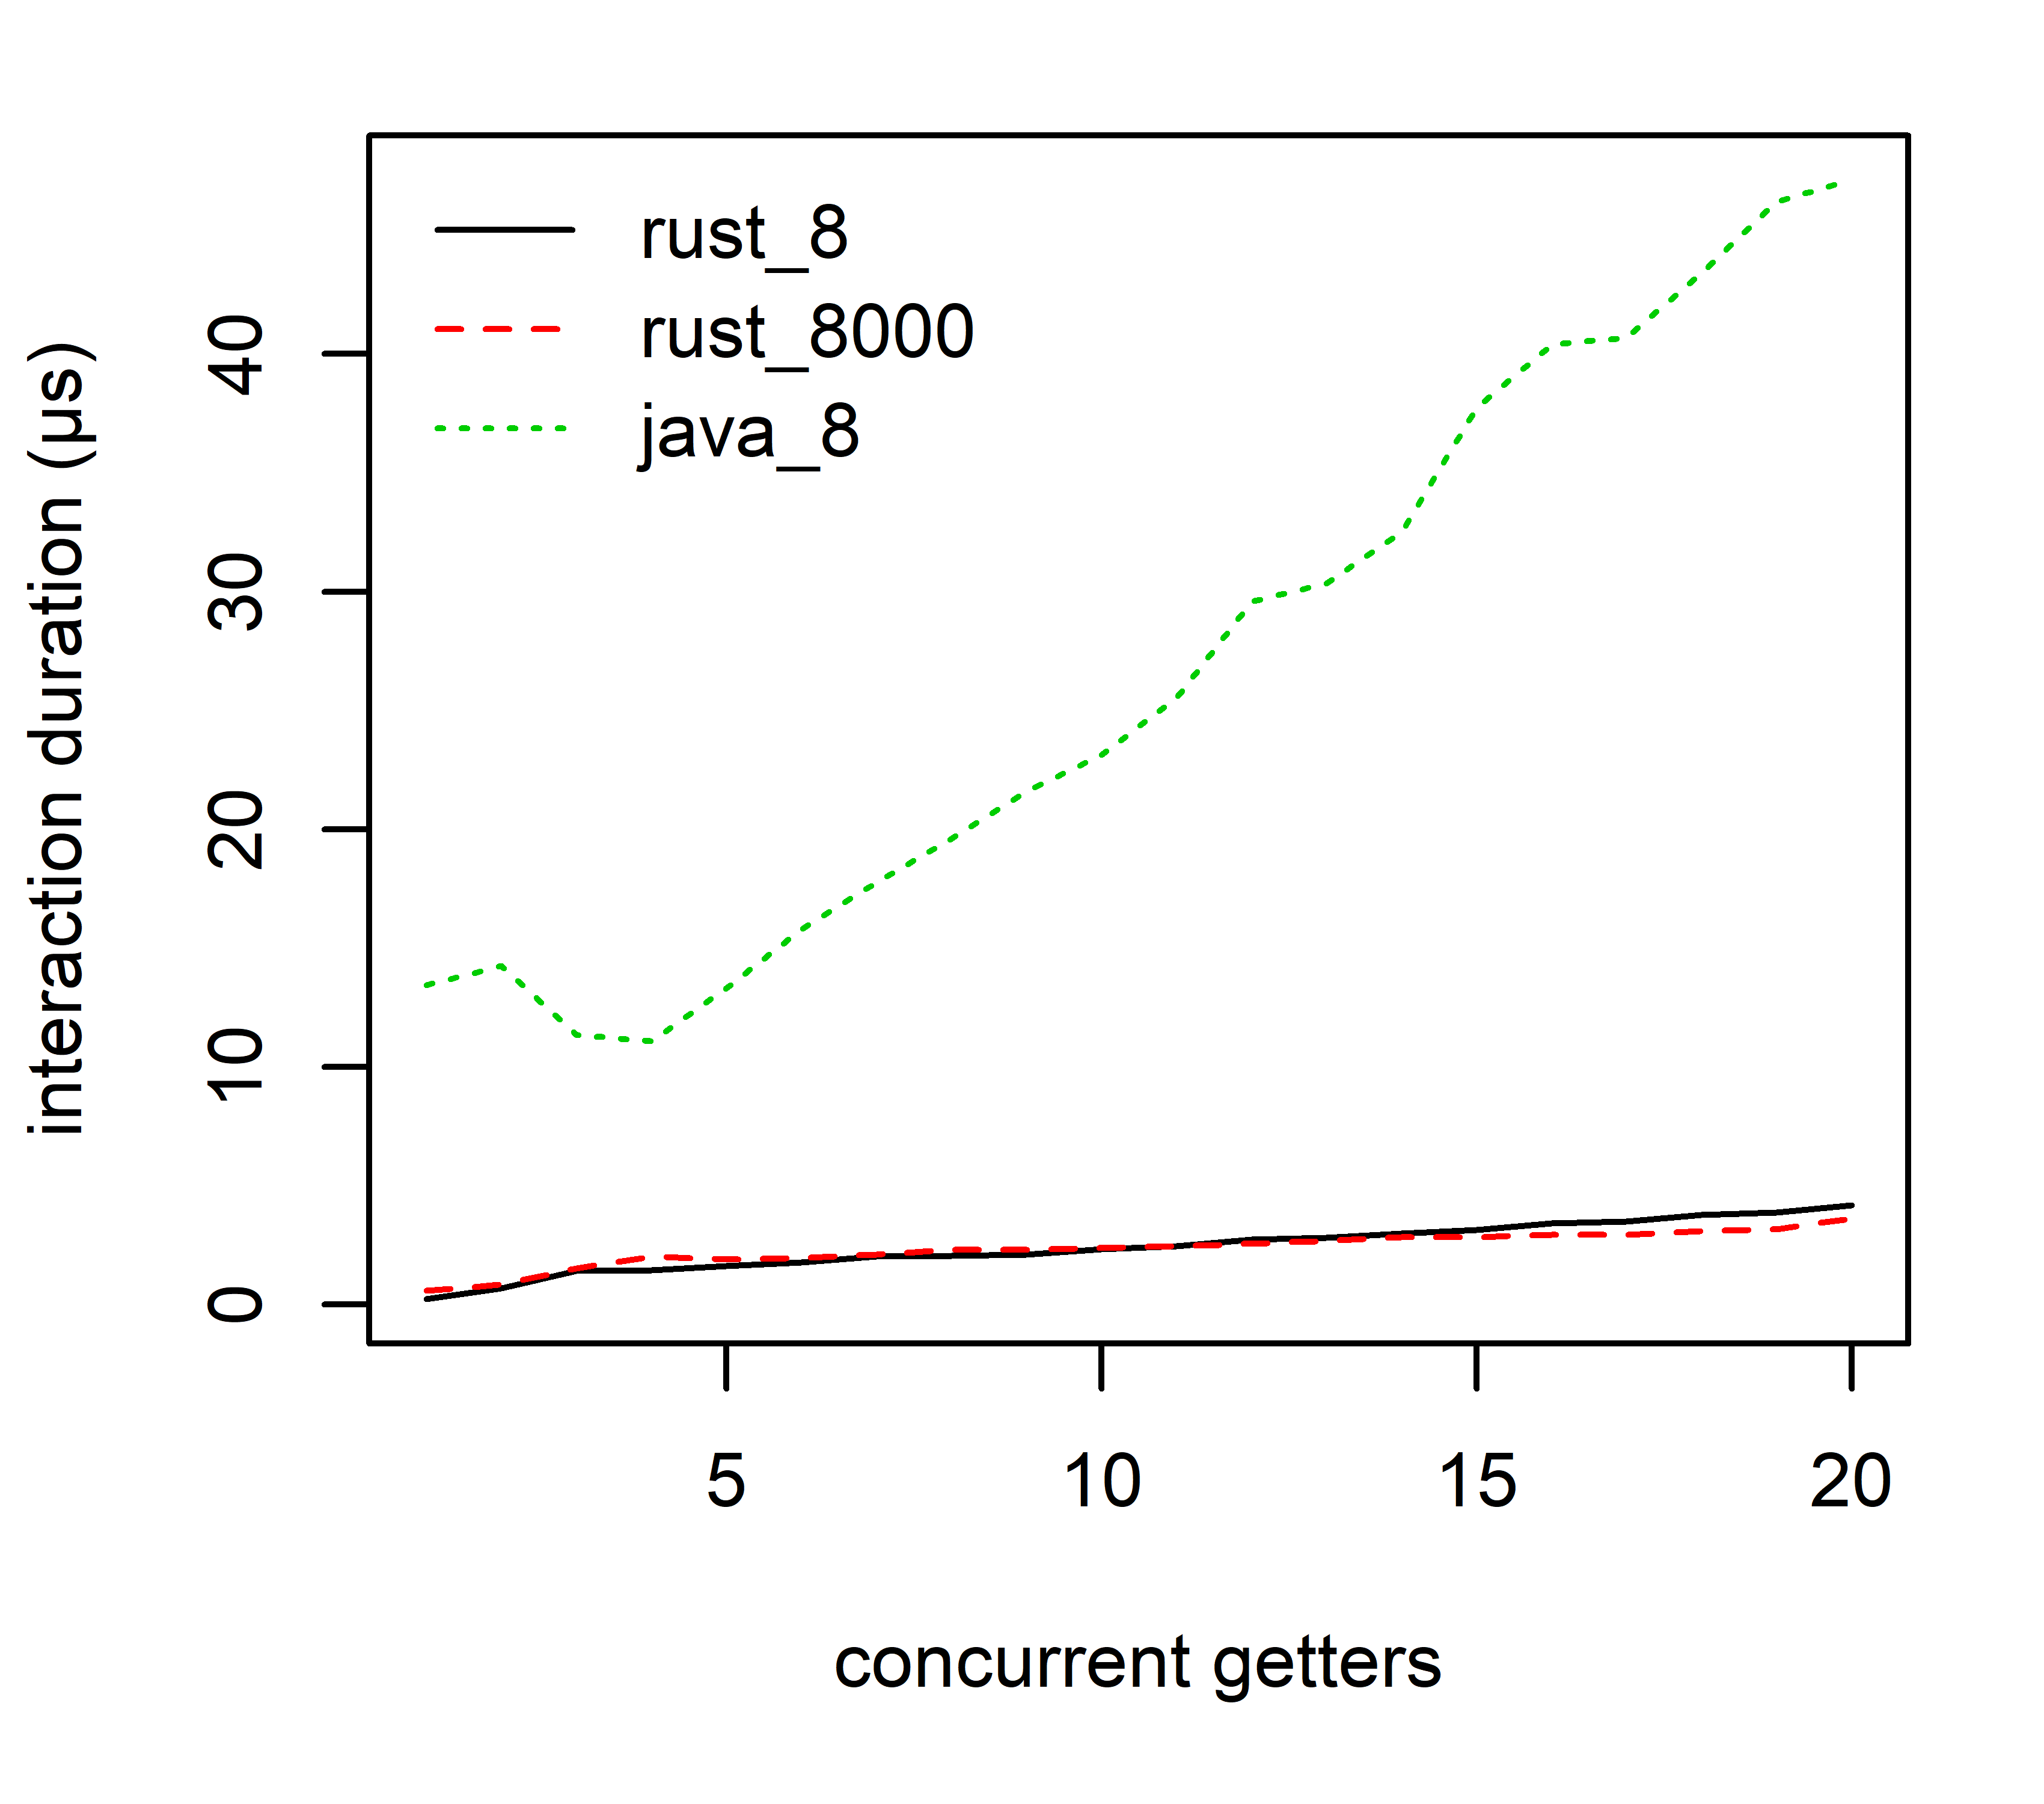
\includegraphics[width=\textwidth]{experiments/rust_v_java_0.png}
			\caption{}
			\label{fig:rust_v_java_0}
		\end{subfigure}%
		\begin{subfigure}[b]{0.63\textwidth}
			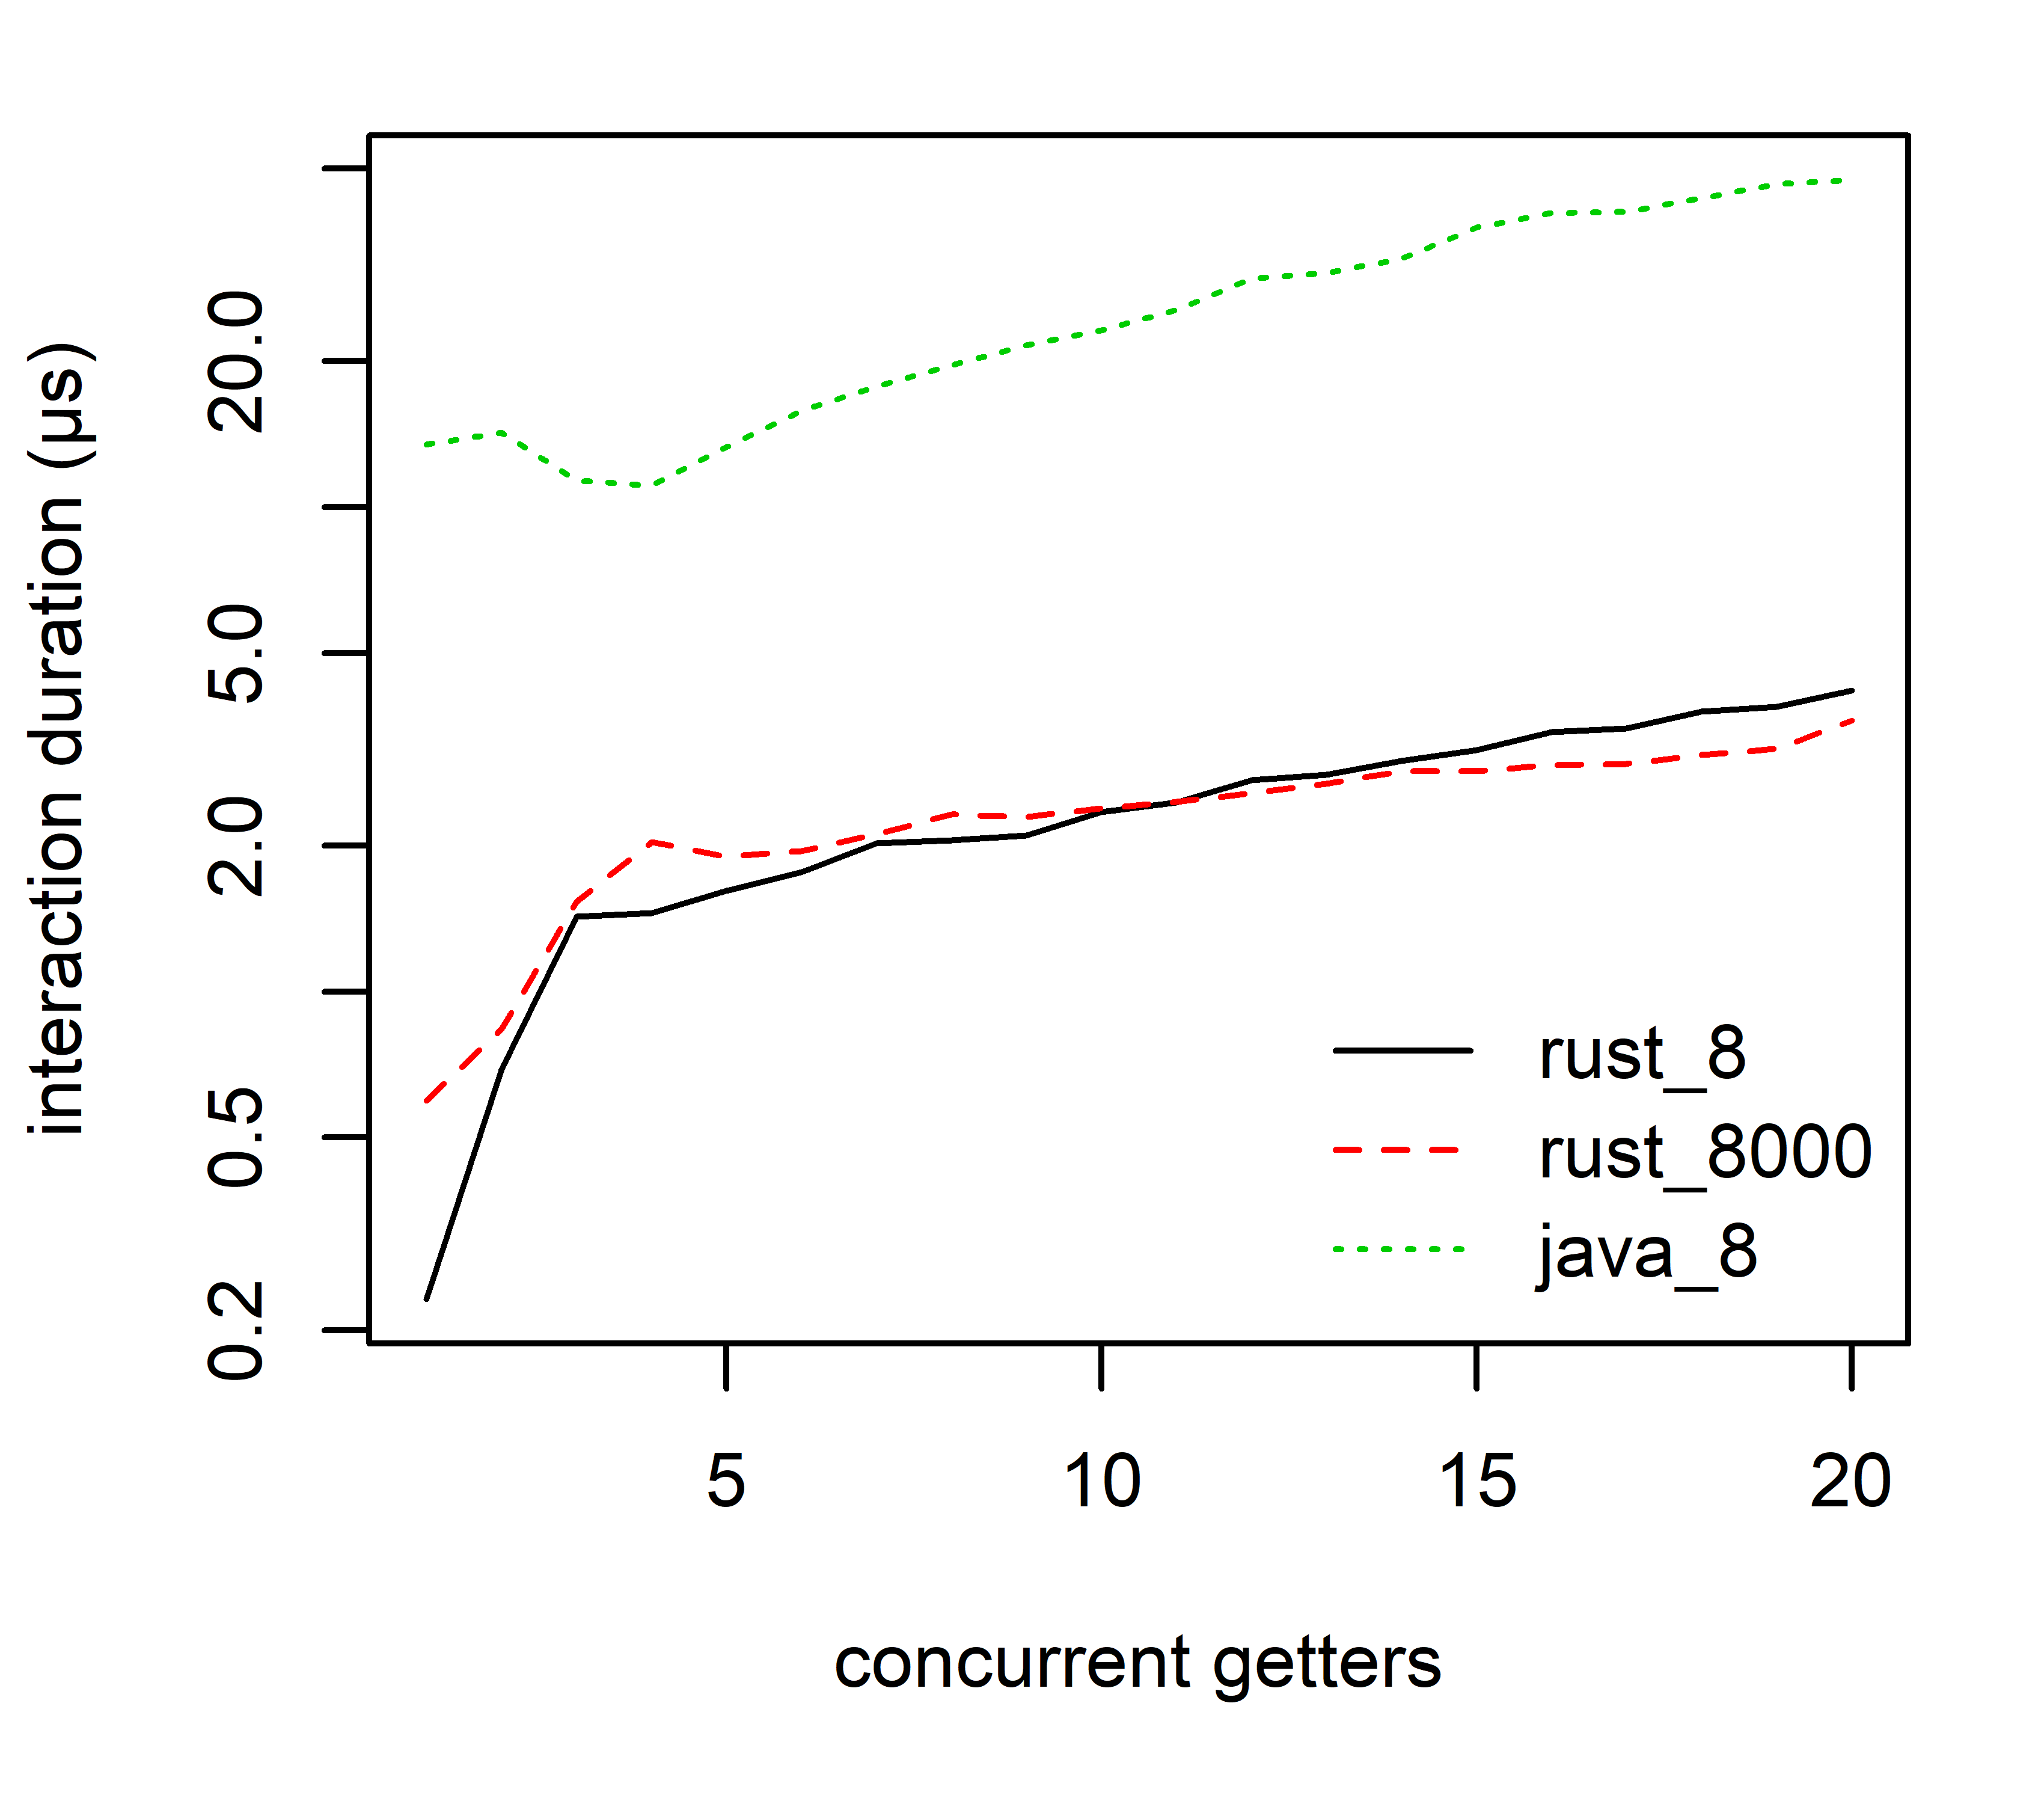
\includegraphics[width=\textwidth]{experiments/rust_v_java_1.png}
			\caption{}
			\label{fig:rust_v_java_1}
		\end{subfigure}%
	}
	\caption[Java vs.\ Rust interaction time for small values.]{Comparison of interaction time for the $fetch$ connector for both Java and Rust backends moving small values. \texttt{rust\_8} and \texttt{java\_8}  both move a payload of 8~bytes (to match the reference size of the 64-bit JVM). \texttt{rust\_8000}  gives an example of how the runtime of Reo-rs can change with respect to modest changes in data size. The two sub-figures mirror one another except for the linear and logarithmic y-axes respectively.}
	\label{fig:rust_v_java}
\end{figure}

The unfairness of our comparison cuts both ways, as there is not a clear means of comparing the transmission of large values; the Java version relies entirely on object aliasing, effectively implementing different semantics. For Java, the size of values transmitted is largely irrelevant. We begin by a comparison on the only common ground; Figure~\ref{fig:rust_v_java_0} shows both Java and Rust are transmitting pointer-sized objects in the $fetch$ connector. Aside from the order of magnitude difference in runtime, we observe a different \textit{shape}. Reo-rs is observed to be significantly faster in the case of a single getter. This is easy enough to explain; the type relied upon for protecting the coordinator's critical region is \code{Mutex} from the \code{parking\_lot} crate, which provides implementations of these kinds of concurrency primitives. \code{Mutex}~is documented as having a `fast path' optimization for when the lock is acquired uncontested. Runs with one getter are thus able to take advantage of this optimization every time.

Figure~\ref{fig:rust_v_java_2} attempts to draw the same comparison as before, but in the case of large data types. The Java-generated protocol objects do not do true value-passing. It is out of the scope of this project to attempt to implement this

\begin{figure}
	\centering
	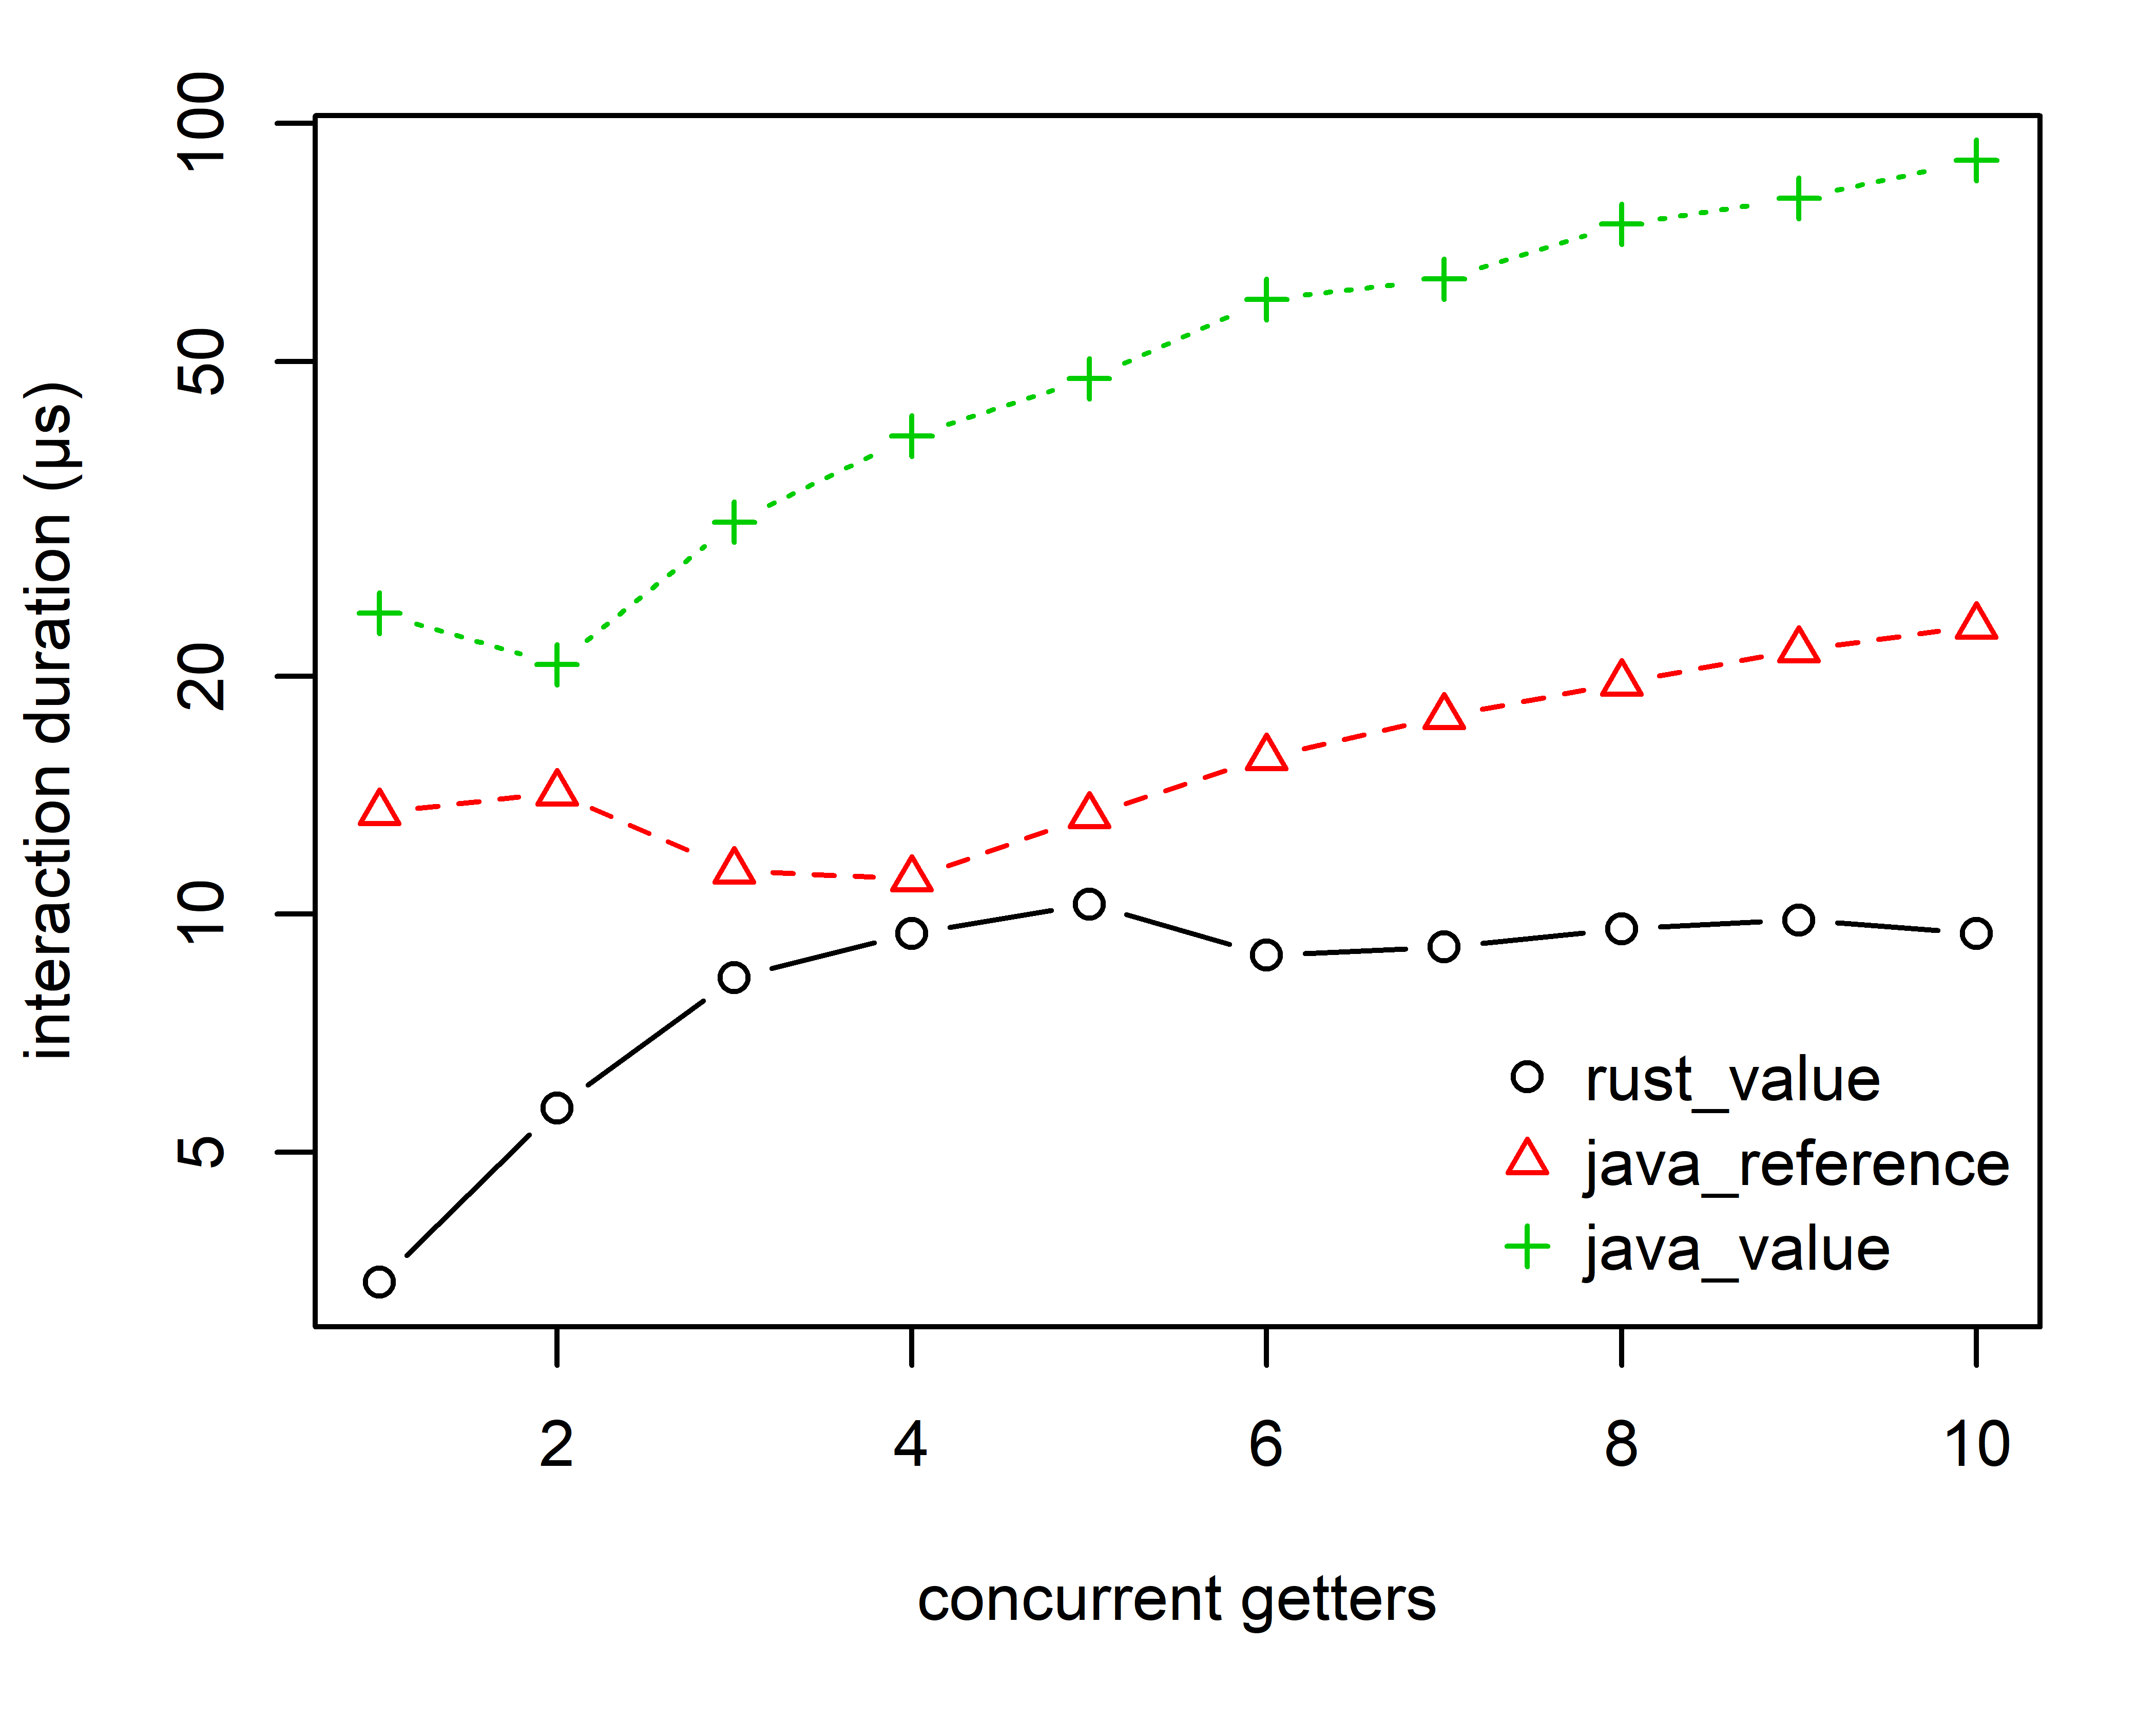
\includegraphics[width=0.80\textwidth]{experiments/rust_v_java_2.png}
	\caption[Java vs.\ Rust interaction time for large values.]{Comparison of interaction time for the $fetch$ connector for both Java and Rust backends moving 64-kilobyte-sized data. The Rust backend moves the datum by value, while the Java parallel \texttt{java\_reference}  aliases the object (moving by reference). This backend does not support value-passing that preserves Reo's semantics. We achieve safety here by the coordinator injecting \code{clone} operations of byte arrays to mirror Rust's bit-wise copy, called \texttt{java\_value} . Note the logarithmic y-axis.}
	\label{fig:rust_v_java_2}
\end{figure}

\subsection{Versus Handcrafted Programs}

Clearly, Reo-rs cannot outperform hand-optimized Rust on a case-by-case basis; whatever Reo-rs does, the hand-optimized code can mimic and specialize to surpass its performance. The utility of the library is to handle arbitrary Reo-generated protocol descriptions, hiding the details away from the user with an API that strikes a balance between flexibility, safety and performance. Here, we attempt to gauge the performance gap between Reo-rs for some small examples of connectors.


Firstly, we examine a case for which Reo-rs is expected to do poorly: we compare the Reo-generated solution of a simple protocol to handcrafted solutions. To make matters worse, we perform the experiment in a circumstance in which explicit synchronization bookkeeping is unnecessary: port operations are accessed sequentially.
Concretely, we examine the $fifo1$ connector. At these small scales, it matters considerably how we perform our optimization. Figure~\ref{fig:exper_rtt} shows runtimes for Reo-rs compared to three handcrafted solutions. \texttt{channel} is the most intuitive solution, relying on the ubiquitous \code{crossbeam} channel for its efficient channels. \texttt{option} uses only the Rust standard library type \code{Option} to act as a memory variable which can be safely written to and read from using its \code{replace} and \code{take} operations. \texttt{copy} uses unsafe Rust and shirks Rust's idioms to write to and read from a pre-allocated heap buffer directly. We see that the runtime of Reo-rs is never the fastest solution. Particularly for small port-values, the simplicity of this protocol is not worth the overhead Reo-rs incurs by traversing rules, comparing guards and so on. Still, it is surprising that Reo-rs overtakes the \code{crossbeam} channel, whose implementation clearly does prioritize the efficient movement of very large values.

\begin{figure}
	\centering
	\makebox[\textwidth][c]{
		\begin{subfigure}[b]{0.63\textwidth}
			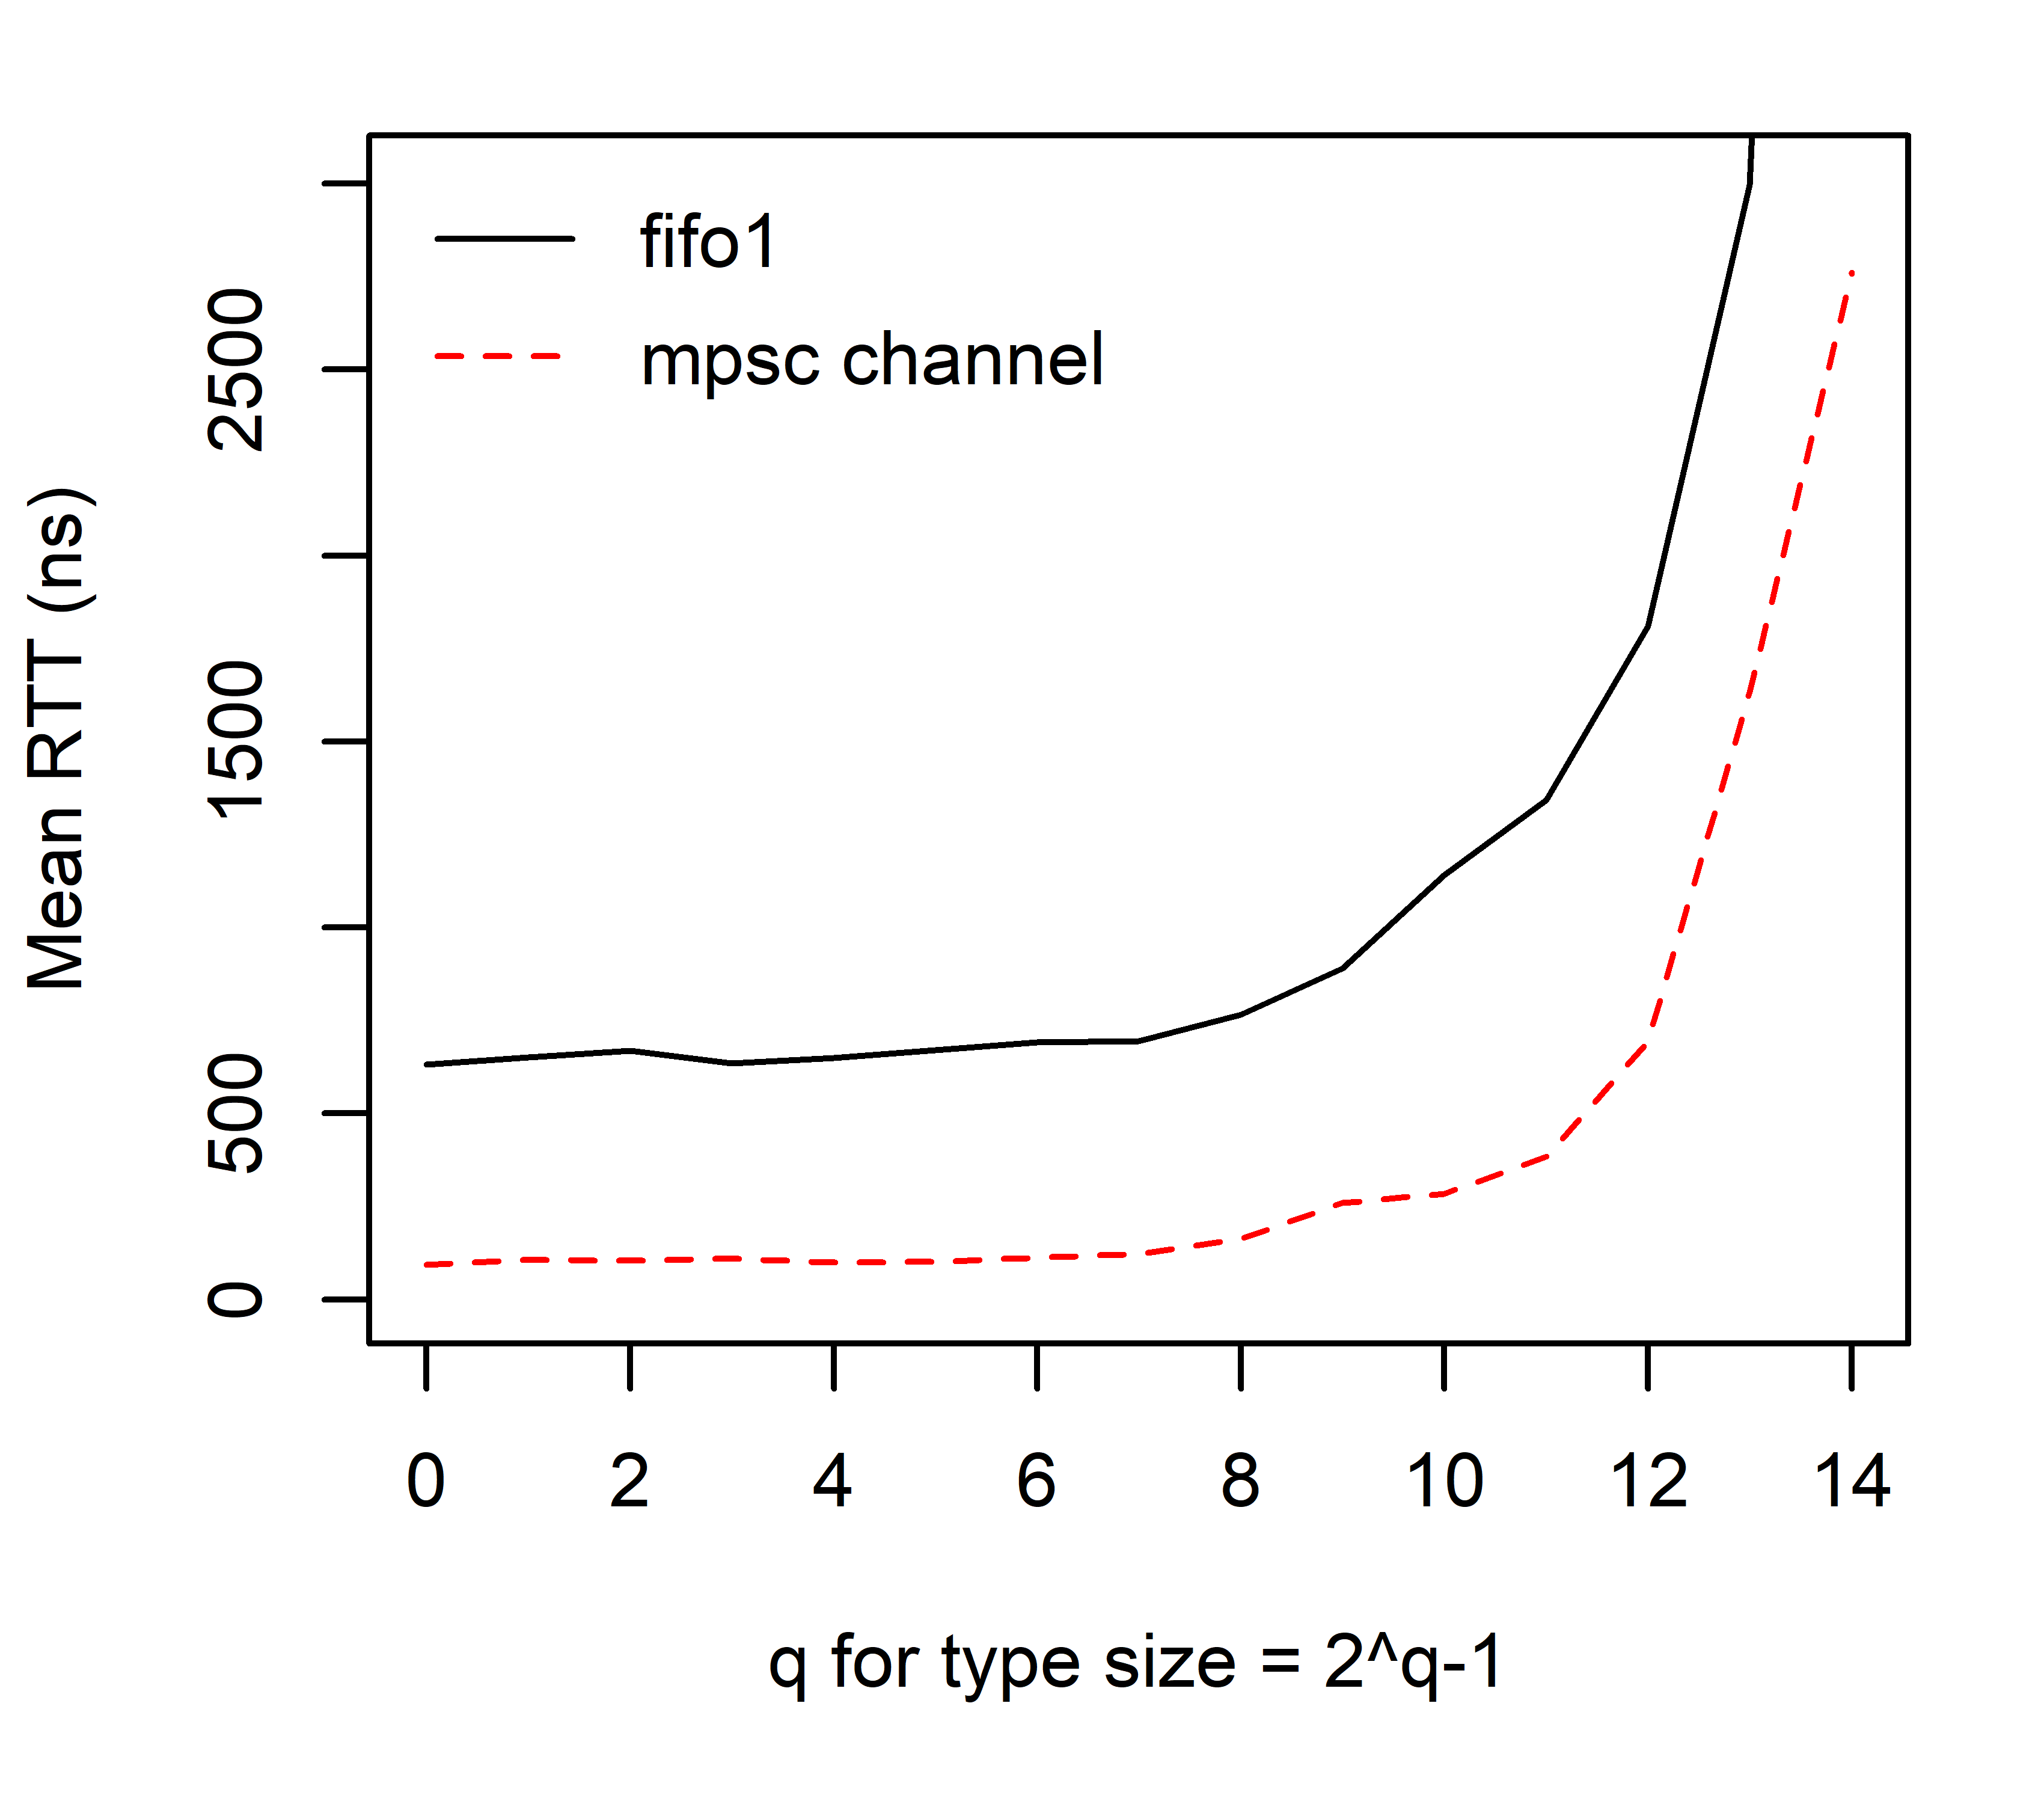
\includegraphics[width=\textwidth]{experiments/rtt_0.png}
			\caption{}
			\label{fig:exper_rtt_0}
		\end{subfigure}%
		\begin{subfigure}[b]{0.63\textwidth}
			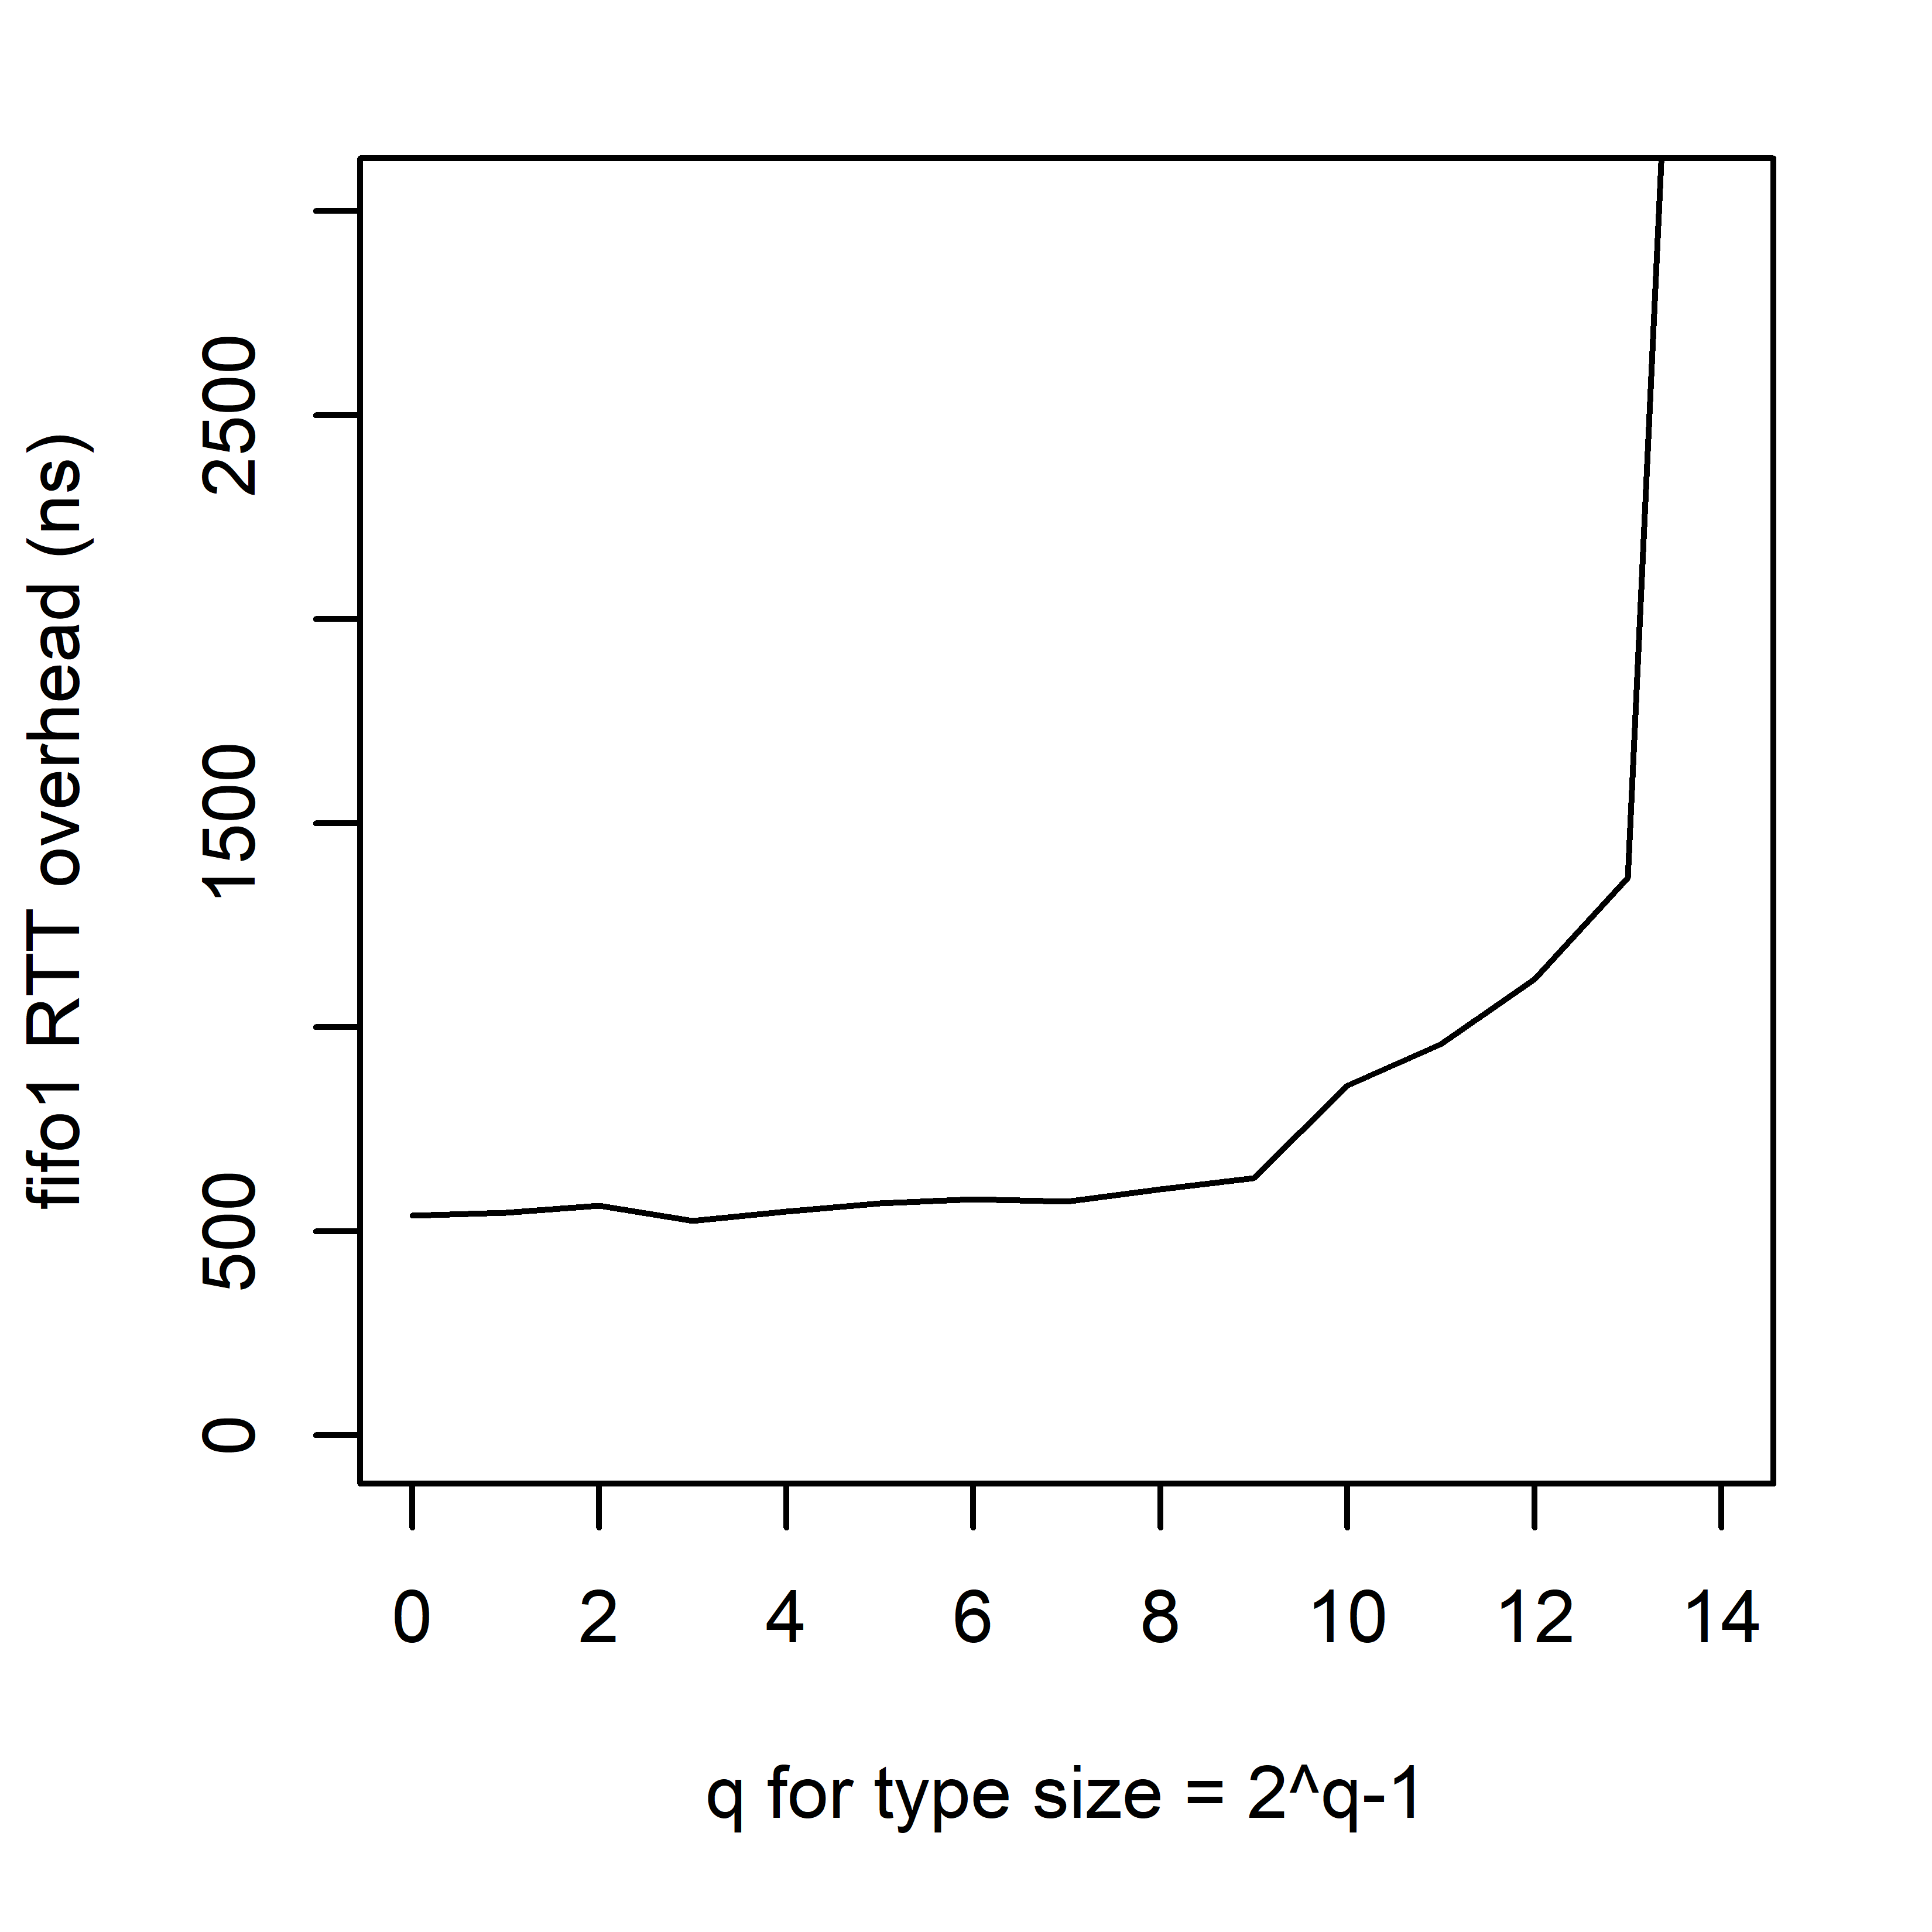
\includegraphics[width=\textwidth]{experiments/rtt_1.png}
			\caption{}
			\label{fig:exper_rtt_1}
		\end{subfigure}%
	}
	\caption[Performance of fifo1 connector vs.\ handcrafted Rust code.]{Time from beginning of \code{put} to end of \code{get} in connector $fifo1$ compared to handcrafted Rust alternatives of various sorts. \texttt{channel} is intuitive, using a \code{crossbeam} 1-capacity buffered channel. \texttt{option} stores the temporary variable in an \code{Option} type, and writes and reads from it using \code{replace} and \code{take} operations. \texttt{copy} uses unsafe rust to perform reads and writes to an allocated heap buffer directly. In both figures, the x-axis is logarithmic. The second plot displays information with a logarithmic y-axis also. Results are the mean of $100\times{}1000$ measurements}
	\label{fig:exper_rtt}
\end{figure}

The comparison become more interesting when we apply Reo-rs to less trivial connectors that make use meaningful synchrony and state. The $alternator2$ is a canonical Reo circuit that routes messages from putters $\{P_0, P_1\}$ to getter $G$ in an alternating fashion (starting with $P_0$). The semantics of this connector are subtly different from that of a $sequencer$; the first value is transmitted once all ports are synchronously ready, and the second value is transmitted asynchronously.

Listing~\ref{fig:alternator2_runtime} shows how Reo-rs fares against a simple handcrafted solution which maps Reo-rs channel primitives and the connector's synchronization constraint to \code{crossbeam}'s channels and the \code{Barrier} in Rust's standard library, implemented to closely correspond with the specification, available for inspection as Listing~\ref{listing:alternator_manual} in the appendix. Figure~\ref{fig:alternator2_runtime_1} shows that, as before, the performance of Reo-rs far surpasses that of our handcrafted solution for very large values, likely as a result of relying on \code{crossbeam}, whose slowdown was previously observed in Figure~\ref{fig:exper_rtt}. More interesting is the observation that while Reo-rs is still inferior for small values, the gap has closed significantly across the board, suggesting that the synchronization overhead is more similar in both versions. For completeness sake, and to put out best foot forward, we include the effects of the C-like \code{unsafe} API variants of Reo-rs port operations explained in Section~\ref{sec:port_operations}.  

The alternator circuit is still simple enough that the handcrafted implementation is only a few lines long. It is in our best interest to compare the performance of Reo-rs to handcrafted solutions closer to the expected level of complexity for the use case of Reo. However, as programs become more complex, it becomes more difficult to design fair `objective' handcrafted programs such that the results are meaningful, as their complexity will increase the opportunities for optimizations. We a more complete analysis of the performance of Reo-rs to handcrafted programs to future work. For now, we conclude that Reo-generated Rust is unlikely to outperform handcrafted programs for protocols at the expected level of complexity, but will be generally competitive.

\begin{figure}
	\centering
	\makebox[\textwidth][c]{
		\begin{subfigure}[b]{0.63\textwidth}
			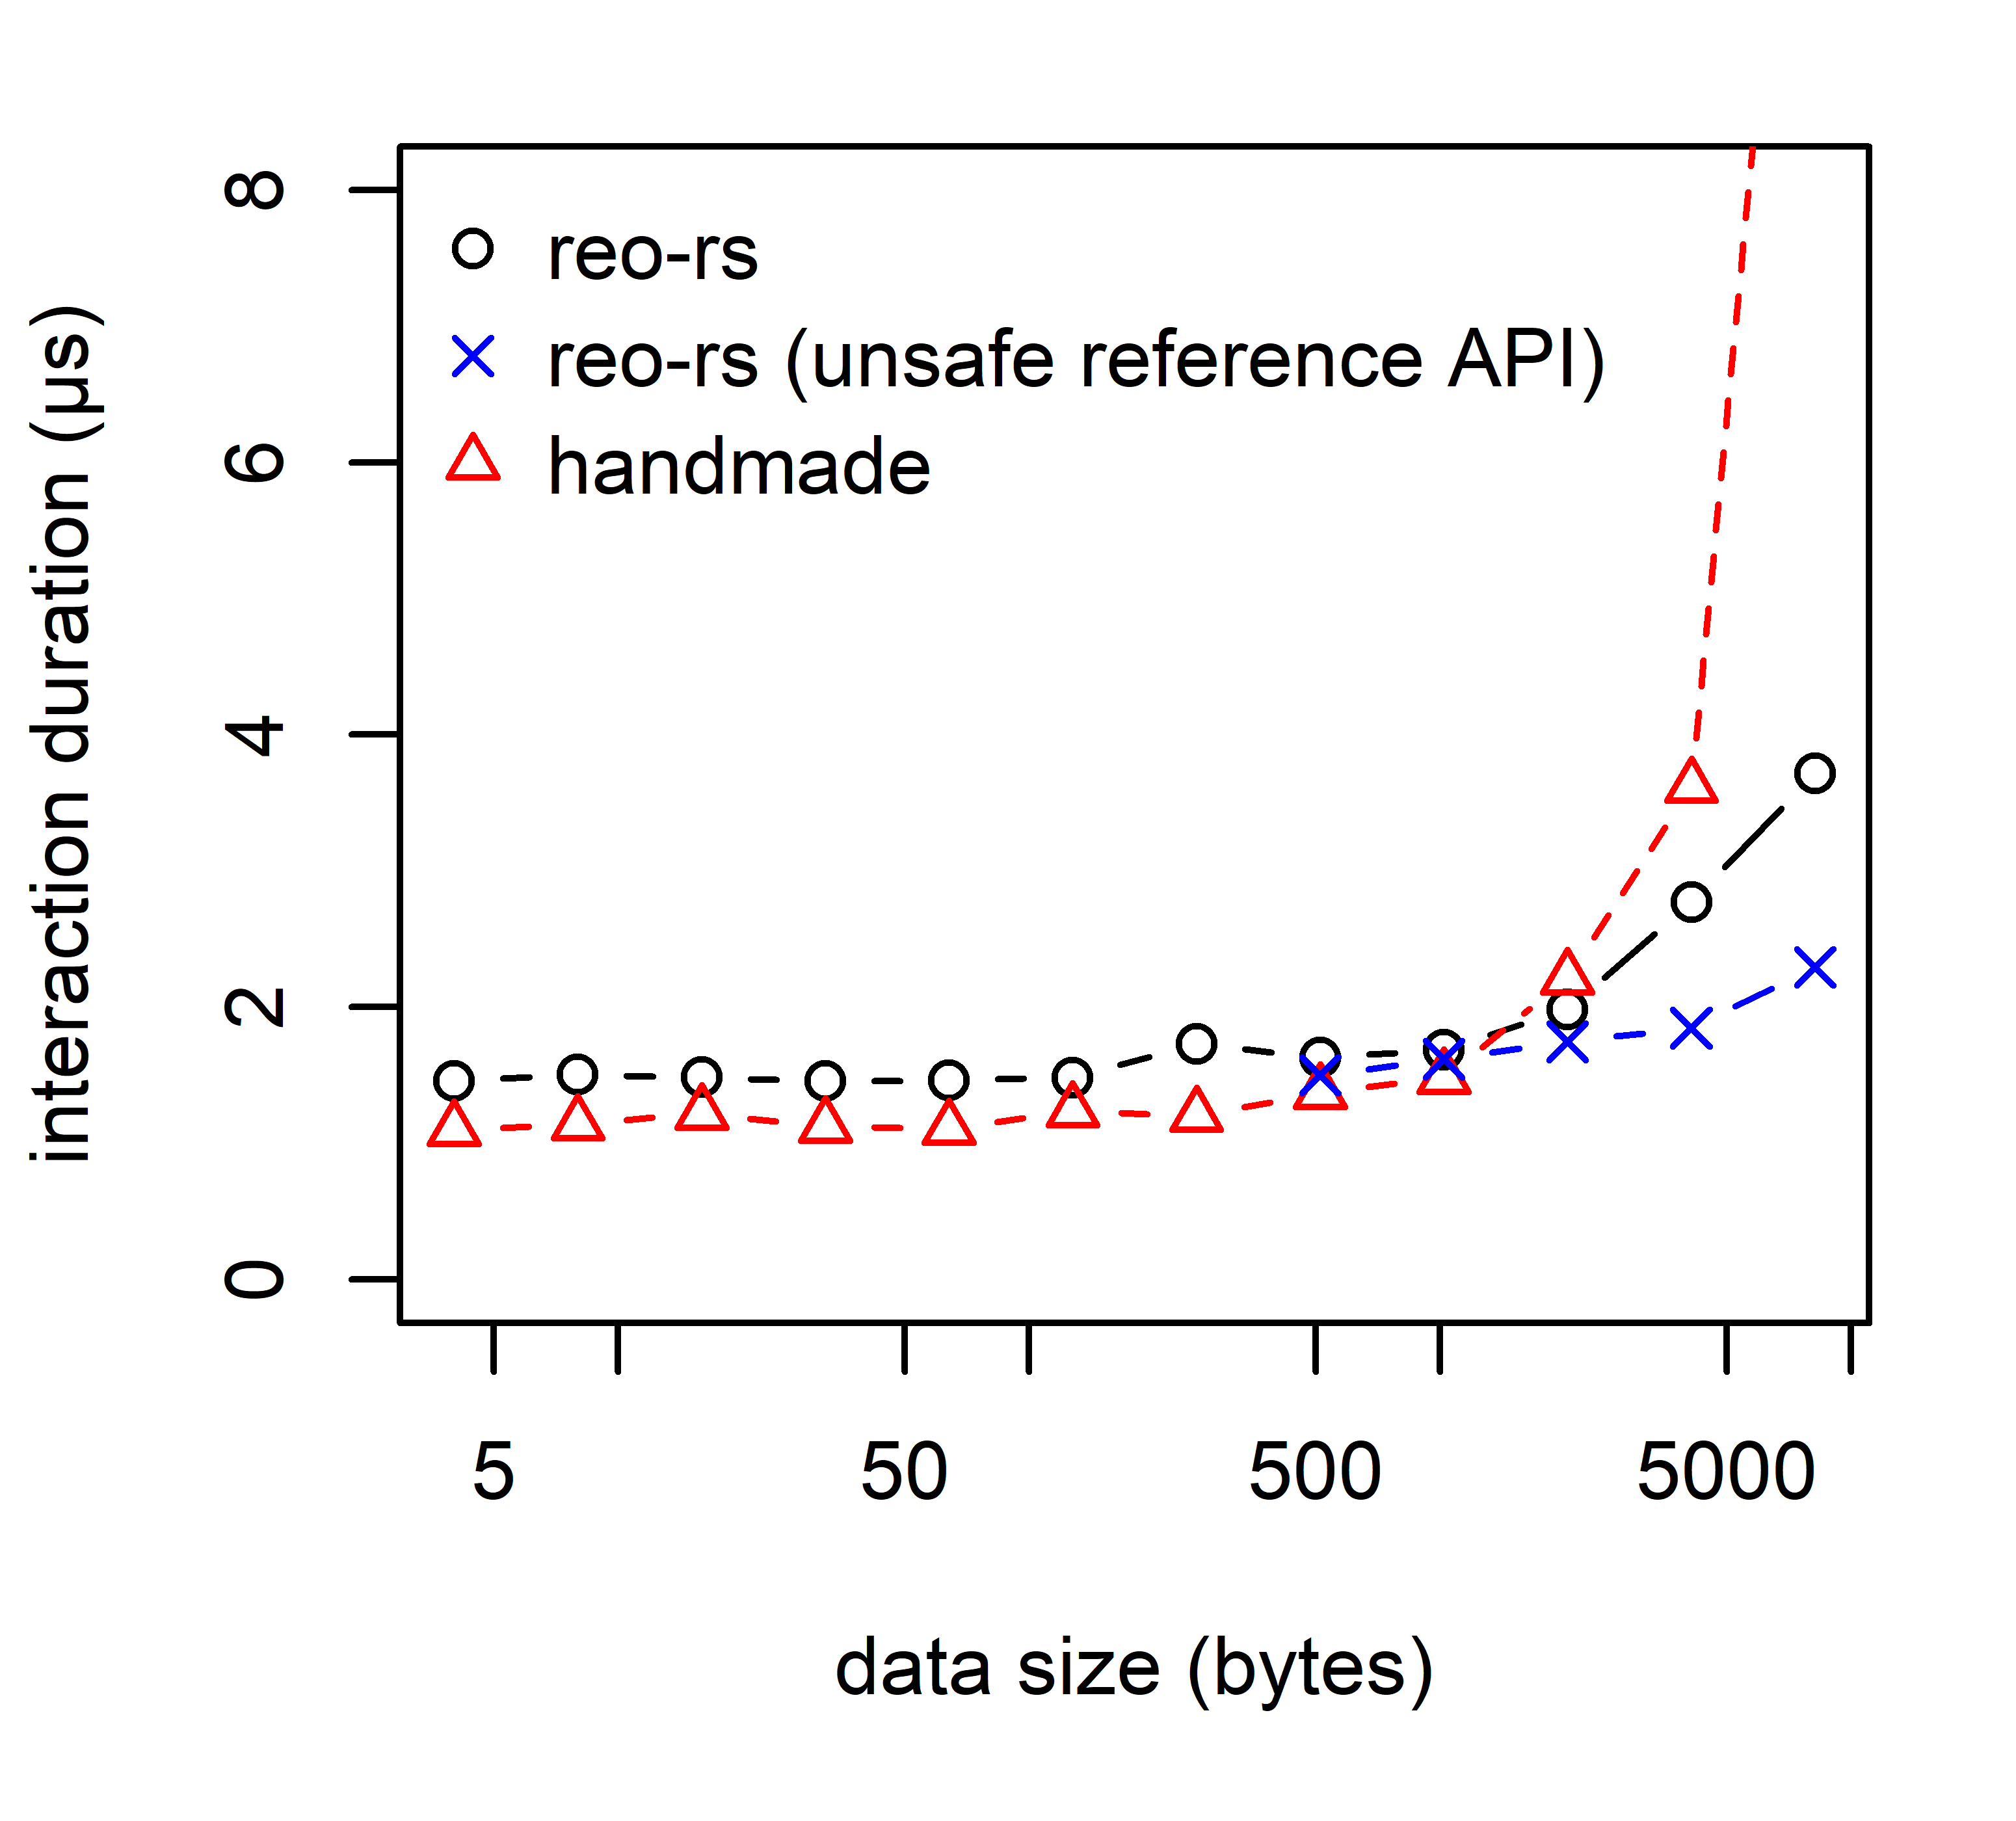
\includegraphics[width=\textwidth]{experiments/alternator_0.png}
			\caption{}
			\label{fig:alternator2_runtime_0}
		\end{subfigure}%
		\begin{subfigure}[b]{0.63\textwidth}
			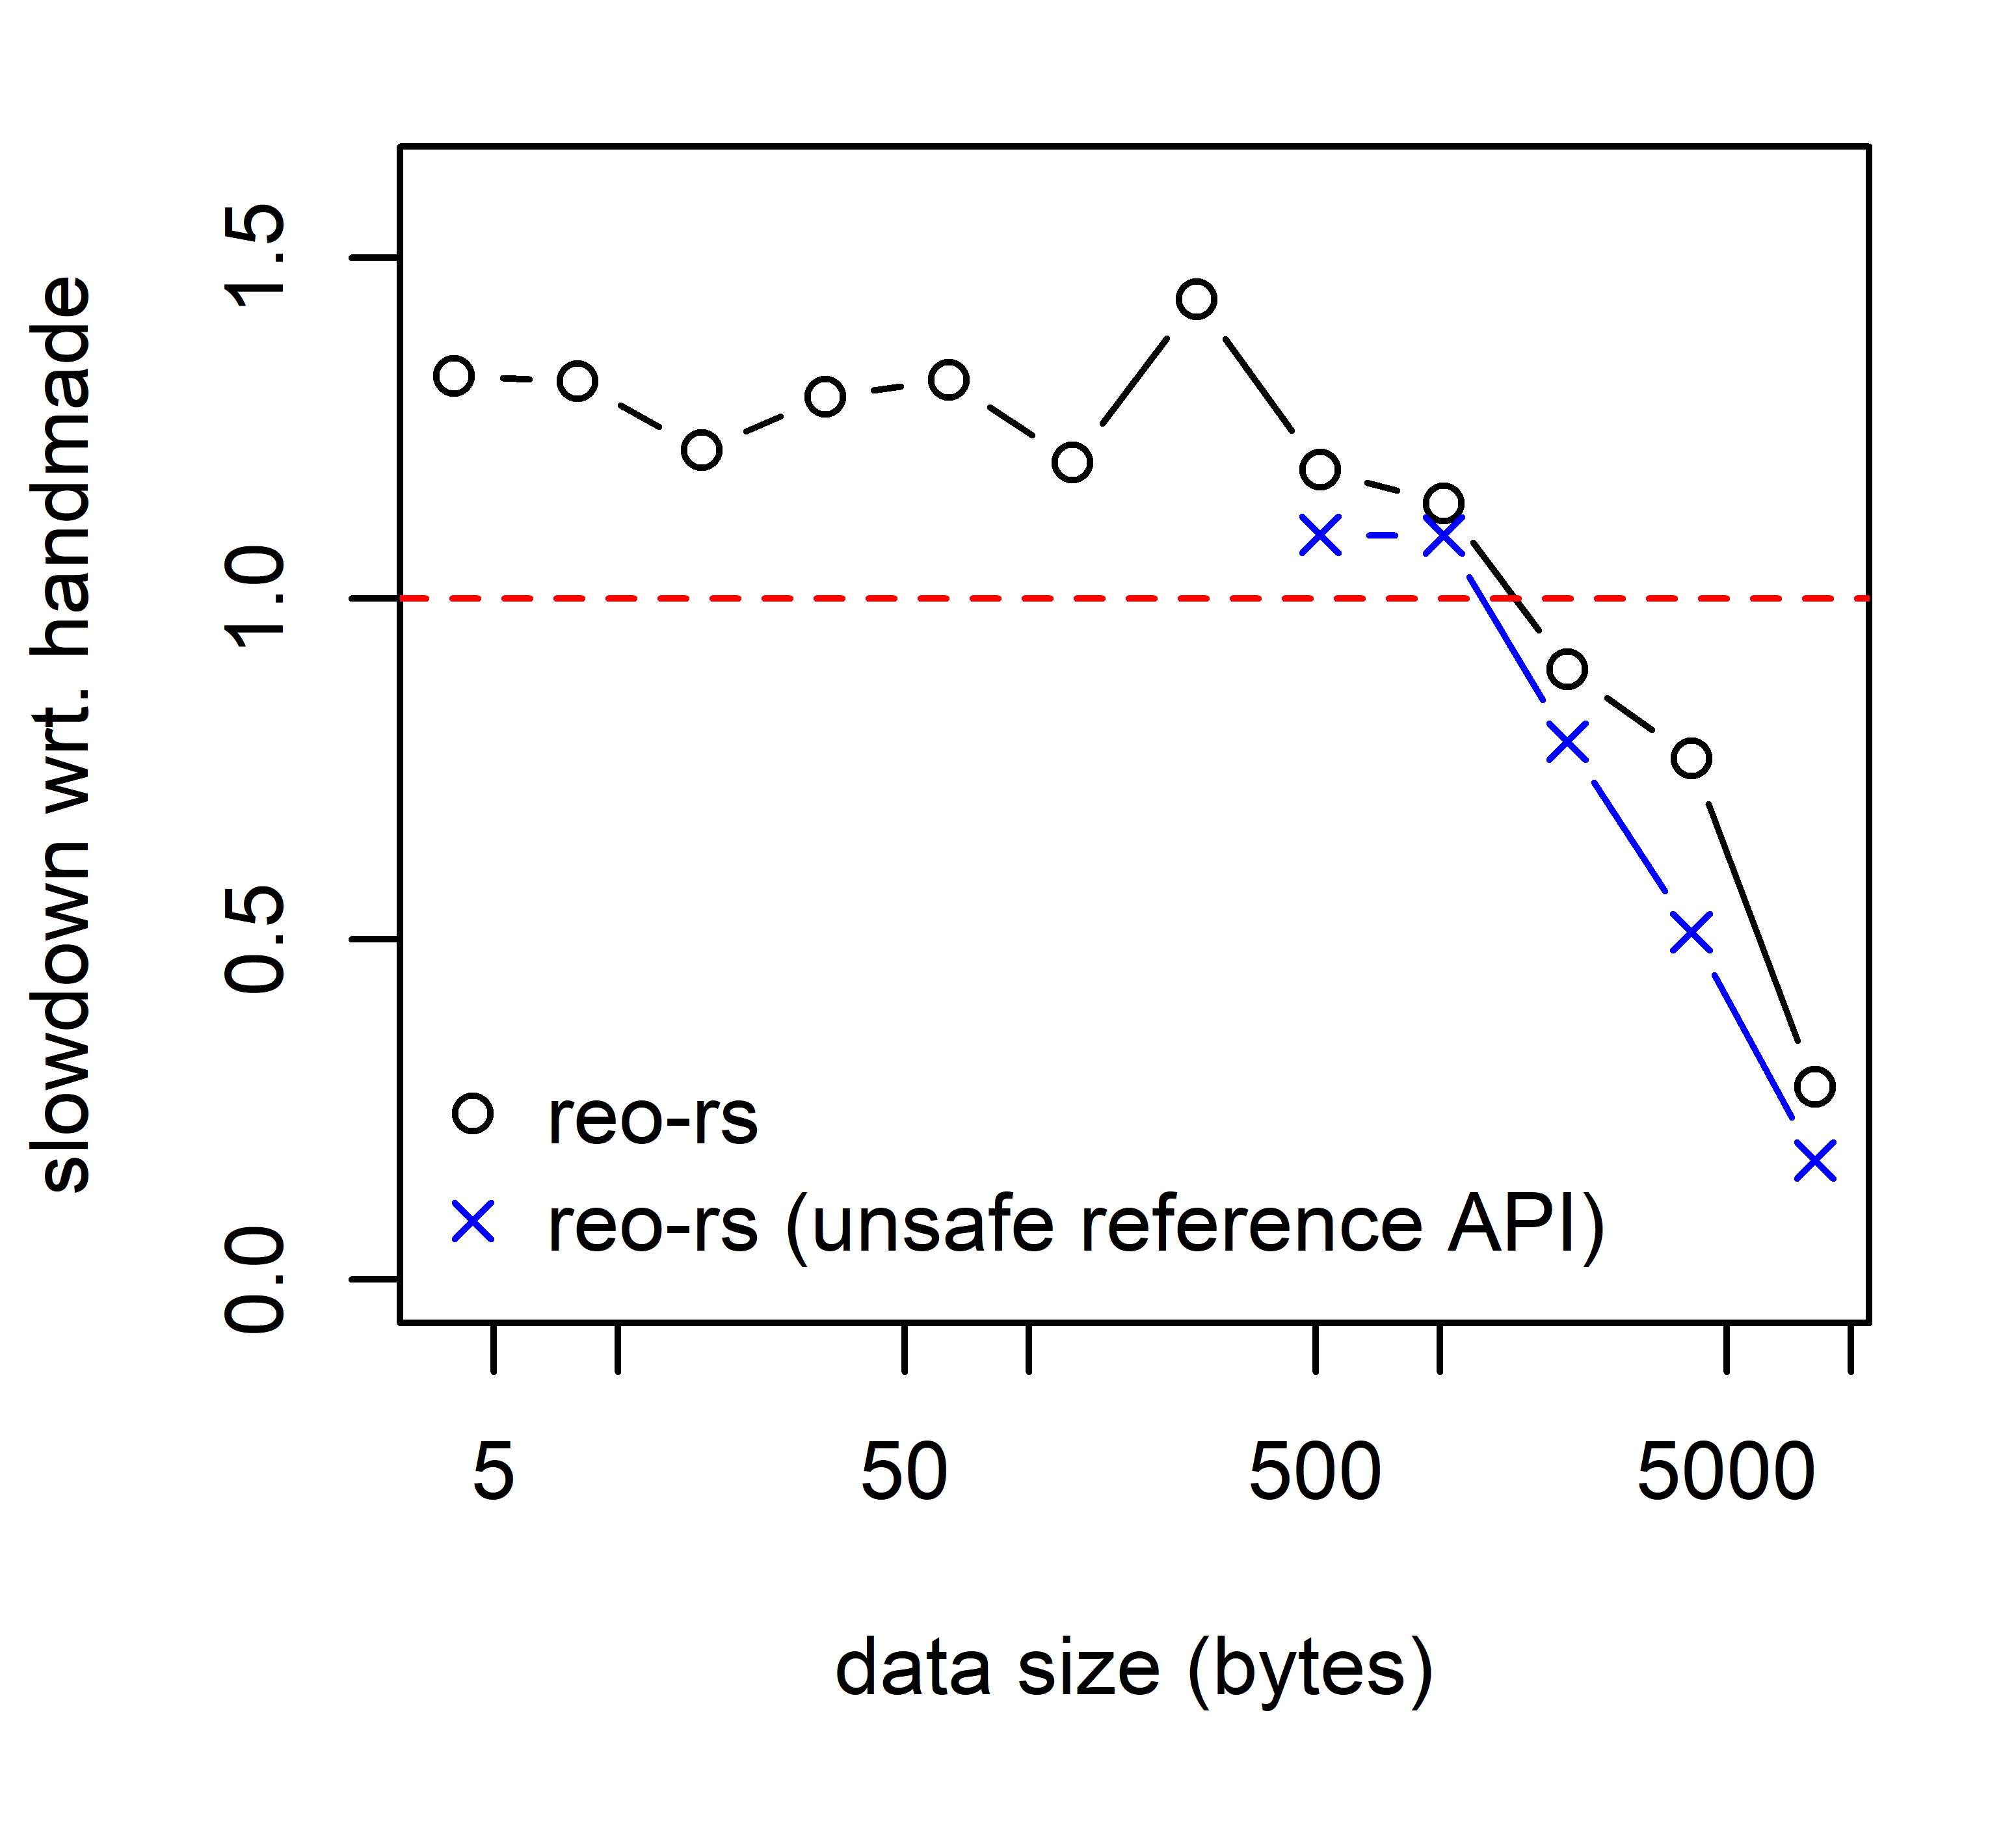
\includegraphics[width=\textwidth]{experiments/alternator_1.png}
			\caption{}
			\label{fig:alternator2_runtime_1}
		\end{subfigure}%
	}
	\caption[Handcrafted vs.\ Reo-generated alternator.]{Mean interaction duration of the Reo-generated $alternator2$ connector in comparison to an intuitive implementation based on channel primitives in the \code{crossbeam} crate, and the \code{Barrier} from the Rust standard library showing (1) absolute runtimes, and (2) the slowdown factor of Reo-rs compared to the handmade code. Note the logarithmic x-axis. Measurements are the mean of $500\times{}5000$ repetitions.}
	\label{fig:alternator}
	\label{fig:alternator2_runtime}
\end{figure}

\section{Overhead Examined}
\label{sec:overhead_examined}
Here, we examine the performance characteristics of Reo-rs in more detail under various circumstances. The goal is to understand how Reo-rs uses its computational resources, and how performance responds to properties of the specific protocol.

\subsection{Parallelism Between Interactions}

For connectors as simple as $fifo1$, overhead is overhead. However, we are particularly interested in understanding how this overhead is partitioned; as connectors become more complex, different parts of this overhead impact parallelism in different ways. Section~\ref{sec:protocol_runtime} explains the nature of the coordinator role, and how its operations are performed holding the lock for the \code{Proto} instance which connects ports as their common communication medium. Table~\ref{tab:active_time} shows measurements for an experiment that attempts to understand which proportion of our overhead is incurred \textit{inside} the critical region, ie.\ by the coordinator. In the case of this experiment, our protocol has rules for movement which can be rendered as a bipartite graph, allowing data flow from any putter in $\{P0, P1, P2\}$ to any getter in $\{G0, G1, G2\}$. As explained in Section~\ref{sec:data_exchange}, movements such as these do not buffer the data elements inside the protocol; getters take values from putters directly. As a consequence, putters are both the first and last to parttake in any of our rule firings' data movements. The table shows the mean duration for which each putter was involved in such a firing. Along with the total duration of the run, we are able to compute to which extent these putters were able to work in parallel. We distinguish between four cases, corresponding to rows in Table~\ref{tab:active_time}. The first three cases do not involve the \code{clone} operation, and are observed to have insignificant differences for all measurements. For this experiment, with modestly-sized values, we conclude that there is no large difference in performance between these three cases:
\begin{enumerate}
	\item [\textbf{move}] Values are moved from putter to getter synchonously.
	\item [\textbf{copy}] Putters retain their values, and getters replicate them with a bit-wise copy that does not mutate the original.
	\item [\textbf{signal}] Getters do not return any data. They return after releasing putters.
\end{enumerate}

The final \textbf{clone} case attempts to observe the effects of intentionally delaying getters outside of the lock by necessitating the use of an explicit \code{clone} operation whose duration is artificially lengthened. At this scale, \code{sleep} calls were out of the question, as its variability overwhelms any meaningful measurements. Instead, \code{clone} perform thousands of chaotic integer computations on the replica before returning it. For these runs, putters retained their original values, but the datum was not marked with the \code{Copy} trait. In all cases, we observed that even at this coarse granularity, there was significant parallelism. For the majority of the time, new rules were able to fire whilst interactions were being completed outside of the critical region. The final case in particular was within a small rounding error of perfect parallelism.

\begin{table}[]
	\centering
	\begin{tabular}{l|lll|ll}
		& \multicolumn{3}{l|}{mean active time} & \multirow{2}{*}{\begin{tabular}[c]{@{}l@{}}run\\ duration\end{tabular}} & \multirow{2}{*}{\begin{tabular}[c]{@{}l@{}}mean\\ parallelism\end{tabular}} \\
		& p0 & p1 & p2 &  &  \\ \hline
		move & 2.68µs & 2.594µs & 2.993µs & 31.1705ms & 2.652 \\
		copy & 2.737µs & 2.4µs & 2.673µs & 28.7161ms & 2.720 \\
		signal & 2.351µs & 2.282µs & 1.943µs & 24.7852ms & 2.653 \\
		\hline
		clone & 4.451ms & 4.461ms & 4.416ms & 44.609s & 2.988
	\end{tabular}
	\caption[Parallelism between getters in runs of the SISO connector.]{Runs of 3~putters greedily sending their 2048-byte data directly to any of 3~getters, 10~000 times. The rightmost column computes how many rule firings were per This test was performed with 4~variants, differing on the properties of the data and whether the putter retained the original. The last column is derived, showing to what extent these putters were able to work in parallel. Measurements are the mean of $100\times{}10~000$ repetitions.}
	\label{tab:active_time}
\end{table}

\subsection{Time Inside the Critical Region}
The previous section, we saw an experiment with data moving between putters and getters. These runtimes included the putter's time spent not only on the movement itself, but also on the time spent in the role of coordinator. Here, we examine the work that pertains to this role and how changes to the definition of rules influence overhead. Figure~\ref{fig:check_time} shows the overhead incurred by a coordinator that traverses unsatisfied rules before finding one to fire. It is apparent that in all cases, the overhead scales linearly, as expected. The time taken to evaluate the satisfaction of a rule varies greatly dependent on its definition; the evaluation of a rule involves many different operations mirroring the intricacies of the imperative form it models, described in Chapter~\ref{sec:imperative_form}. To represent the possibility space, the figure shows measurements for a simple protocol which encounters replicas of one unsatisfied rule repeatedly, where its nature comes in four distinct variants:
\begin{enumerate}
	\item [\textbf{guard}] A rule where some port is not ready. This is detected almost immediately by cheap bit vector operations, as explained in Section~\ref{sec:minimizing_the_bottleneck}. Evaluation takes 8.76ns.
	
	\item [\textbf{false}] A rule whose first instruction checks the predicate $false$. Evaluation takes 18.91ns.
	\item [\textbf{ands}] A rule whose first instruction is a tree-like formula structure of twenty-five conjunctions, only the last of which is $false$. Evaluation takes 180.72ns.
	\item [\textbf{alloc}] A rule whose first instruction allocates a temporary $false$ value. The second instruction checks that this temporary value is true. Upon failure, the allocation must be rolled back, discarding the temporary value. Evaluation takes 316.51ns.
\end{enumerate}


\begin{figure}
	\centering
	\makebox[\textwidth][c]{
		\begin{subfigure}[b]{0.63\textwidth}
			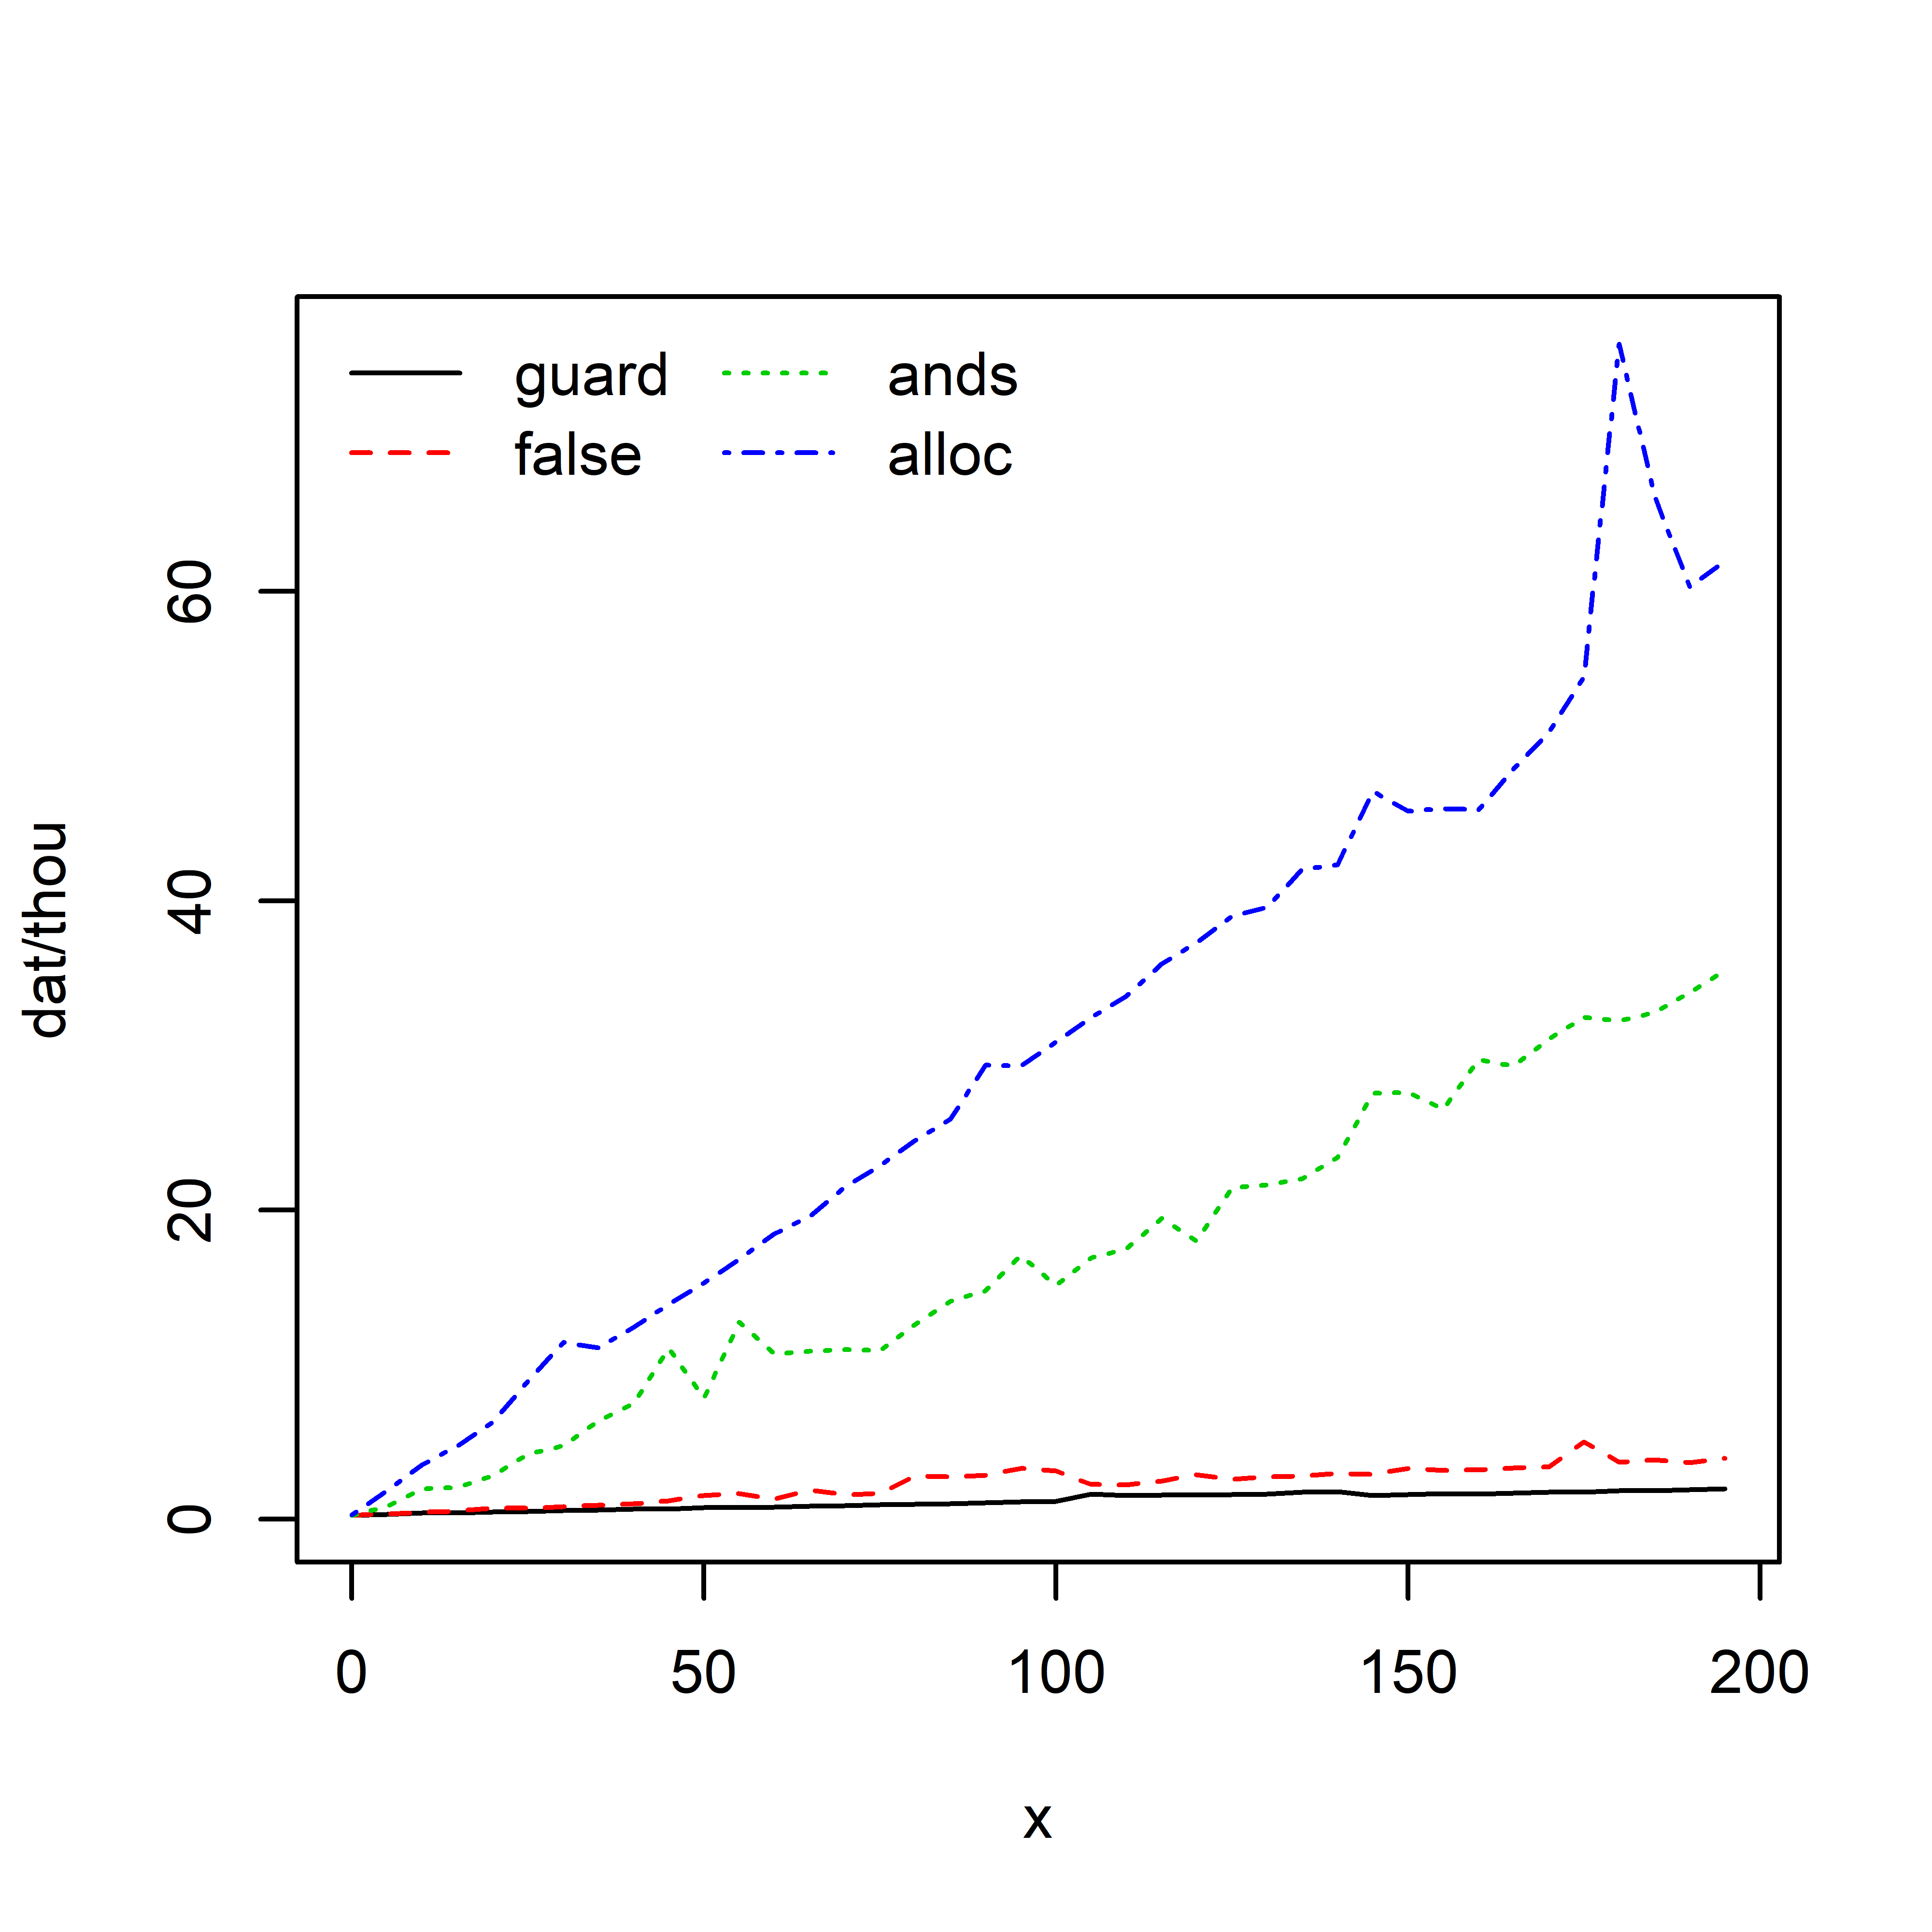
\includegraphics[width=\textwidth]{experiments/check_time_0.png}
			\caption{}
			\label{fig:check_time_0}
		\end{subfigure}%
		\begin{subfigure}[b]{0.63\textwidth}
			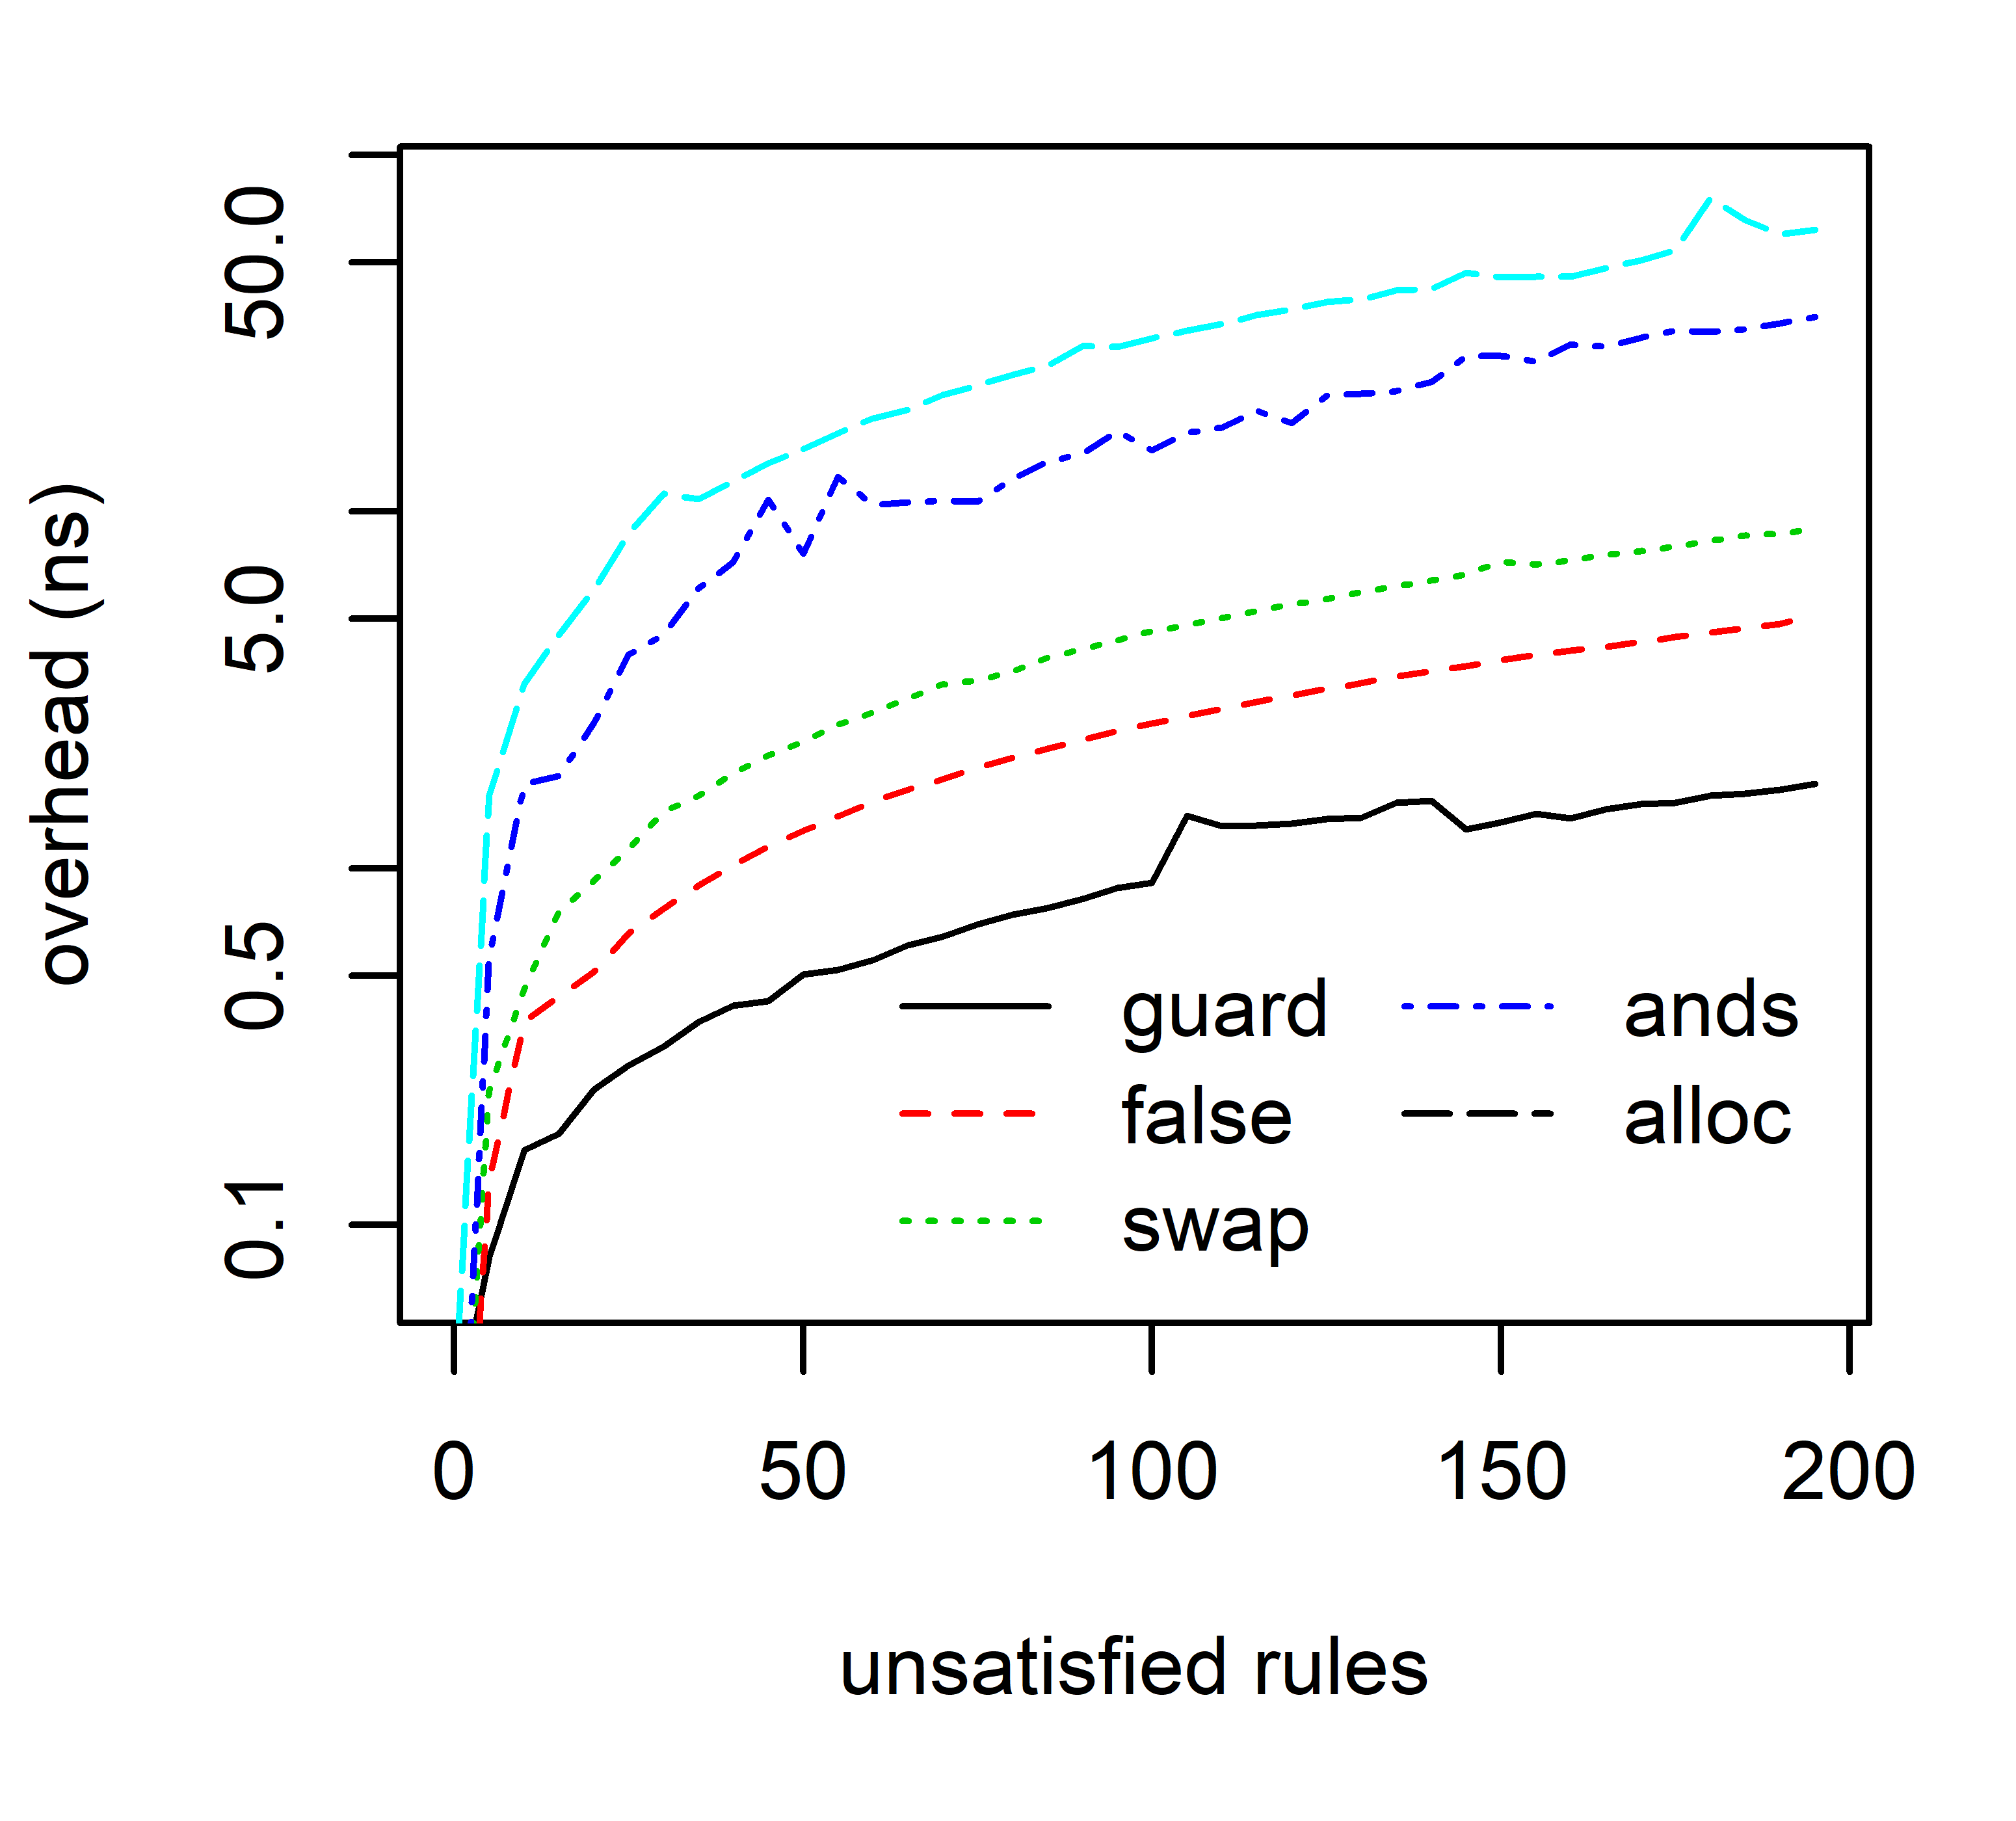
\includegraphics[width=\textwidth]{experiments/check_time_1.png}
			\caption{}
			\label{fig:check_time_2}
		\end{subfigure}%
	}
	\caption[Overhead of evaluating unsatisfied rules.]{Overhead as a result of evaluating a sequence of identical unsatisfied rules before firing something. Experiment is repeated for four variants of unsatisfied rules varying in the complexity of the operations they before before being deemed unsatisfied. The two sub-figures show the same information, with (b) representing it with a logarithmic y-axis to accentuate the small-scale differences. Measurements are the mean of $100\times{}10~000$ repetitions.}
	\label{fig:check_time}
\end{figure}

These results meet our expectations. Rules can be arbitrarily complex, and perform an arbitrary amount of work before concluding that they are not satisfied, and will not fire. Even for this small set of relatively simple examples, we are able to see orders of magnitude in difference between the best case (in which the rule is skipped as early as possible by evaluating a bit-vector), to the worst case (involving several complex instructions). Fortunately, realistic Reo connectors will be defined almost entirely by rules that are either skipped as a result of evaluating these bit-vectors, or not at all. Even more expensive guards can expect to incur overhead in the order of nanoseconds as long as they involve no more than a handful of reasonable instructions. 

\begin{figure}
	\centering
	\makebox[\textwidth][c]{
		\begin{subfigure}[b]{0.63\textwidth}
			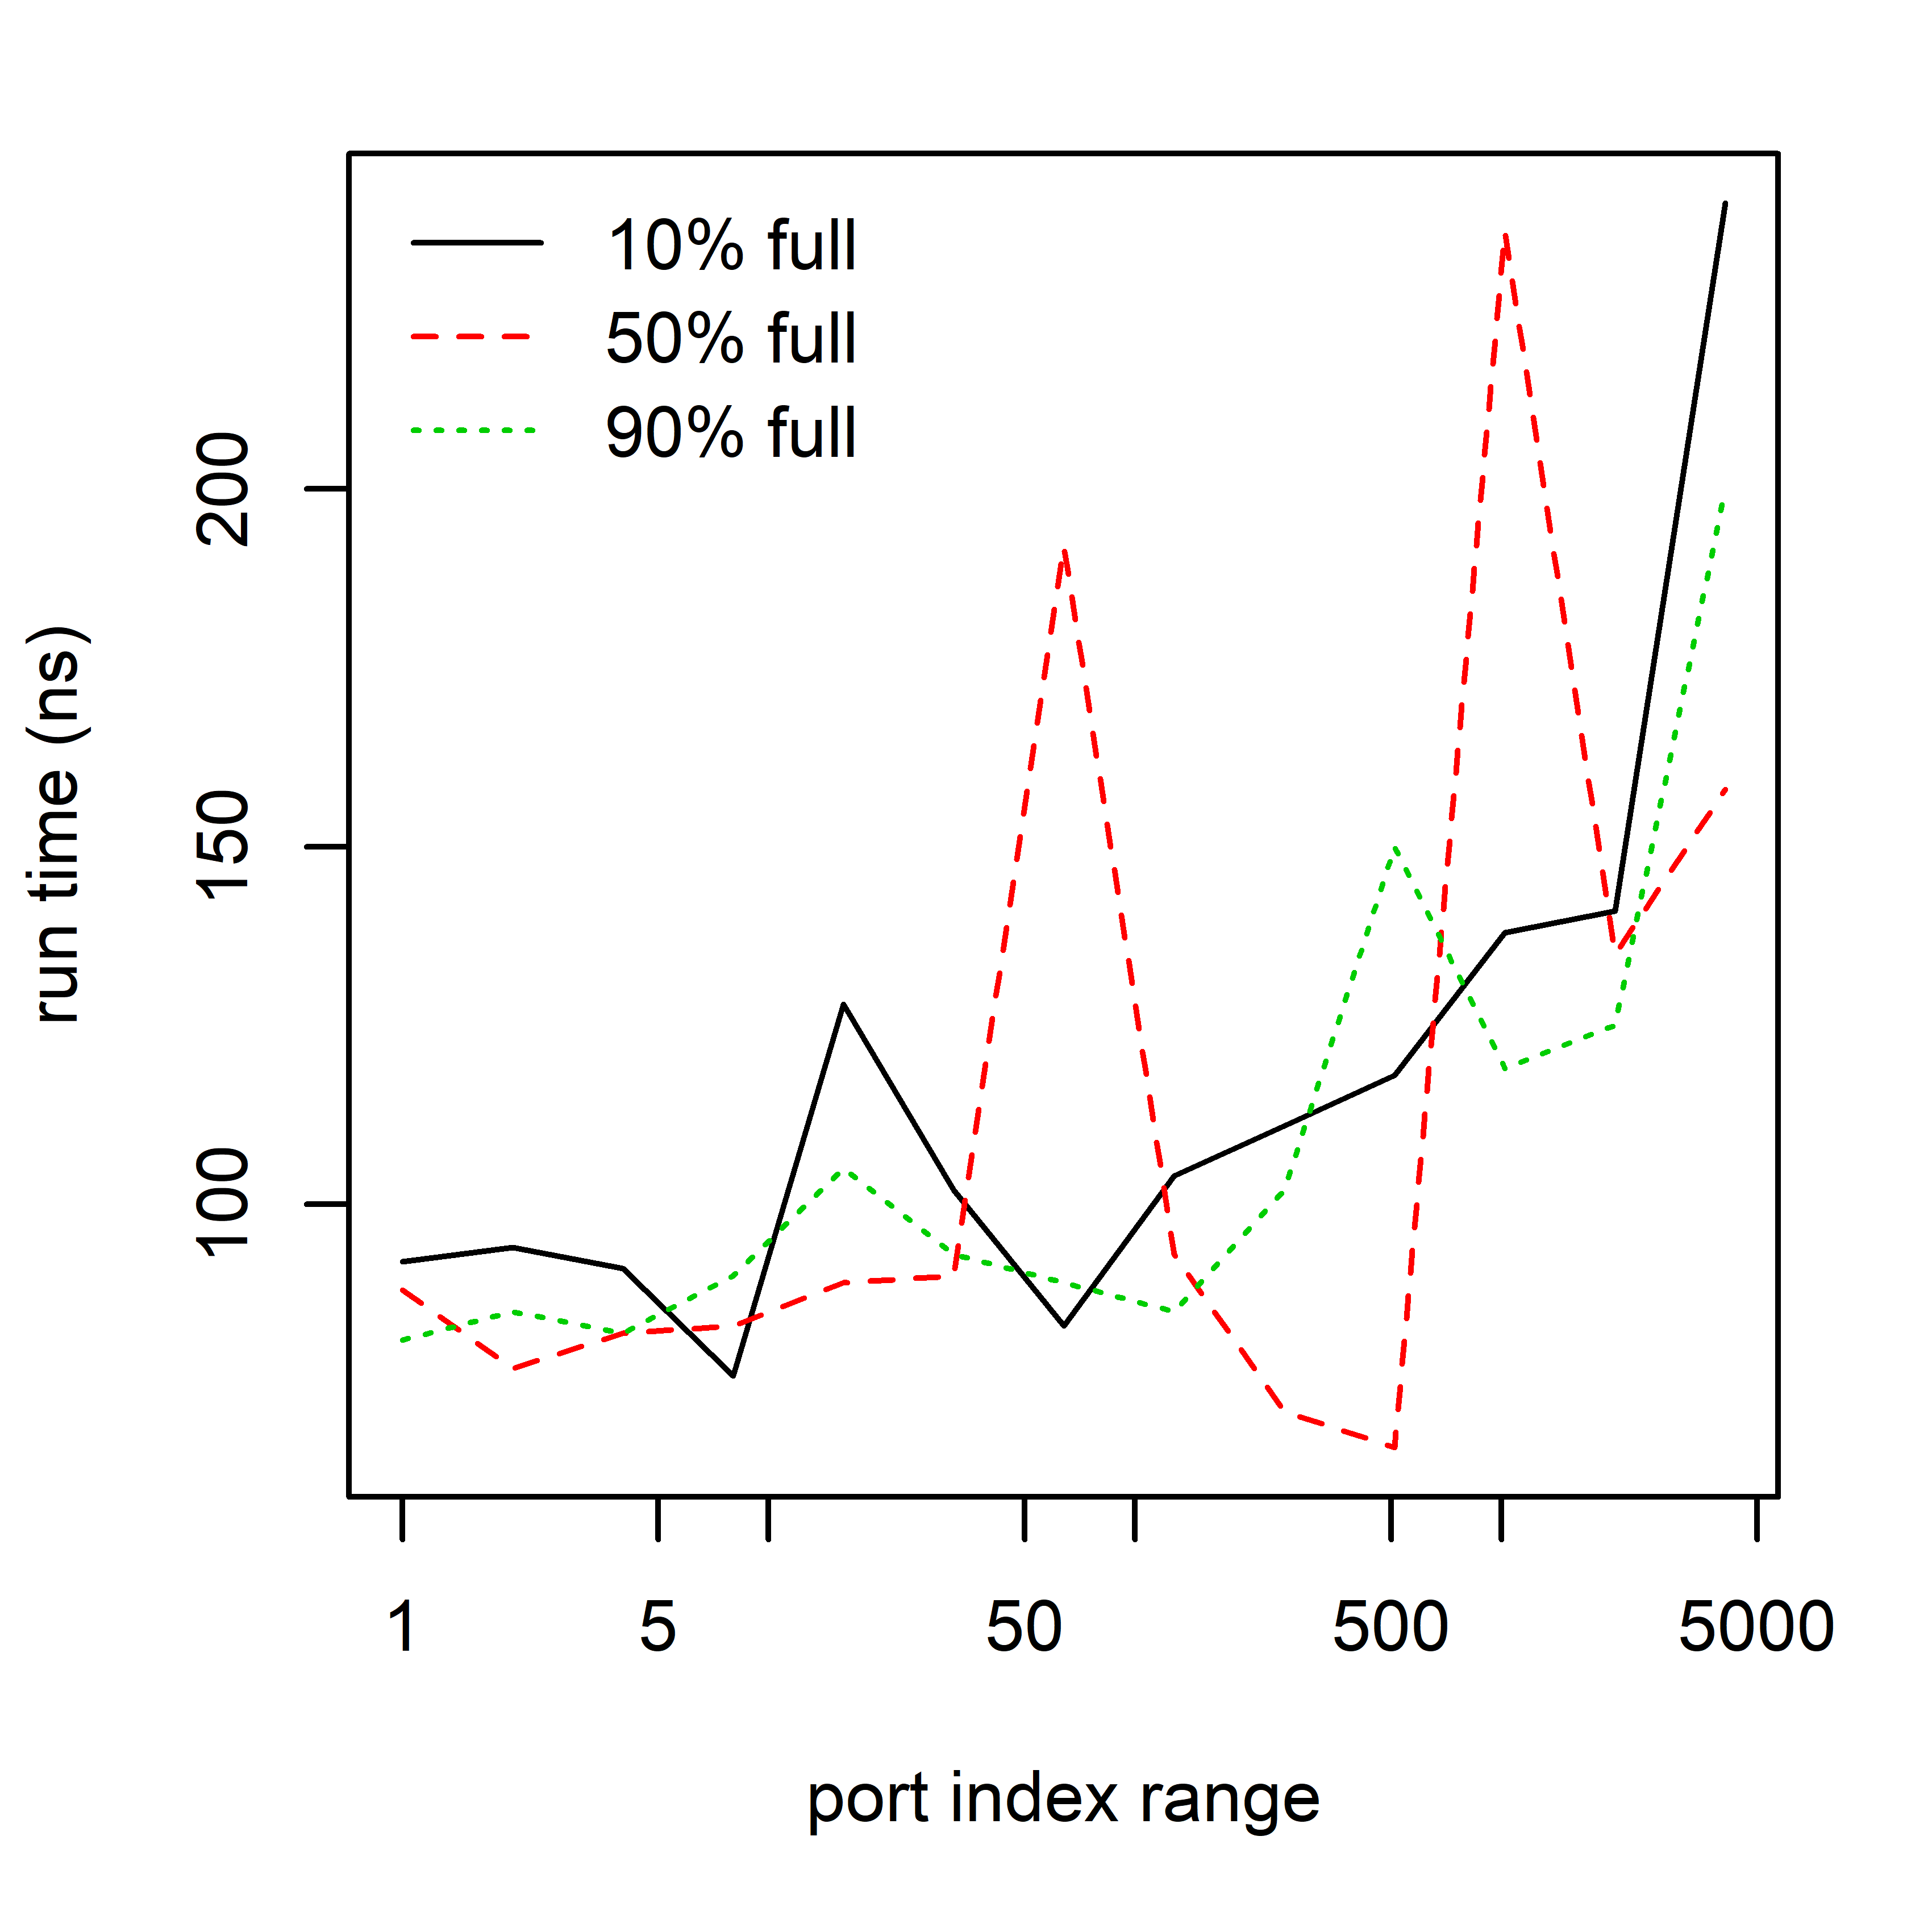
\includegraphics[width=\textwidth]{experiments/bits_0.png}
			\caption{}
			\label{fig:bits_0}
		\end{subfigure}%
		\begin{subfigure}[b]{0.63\textwidth}
			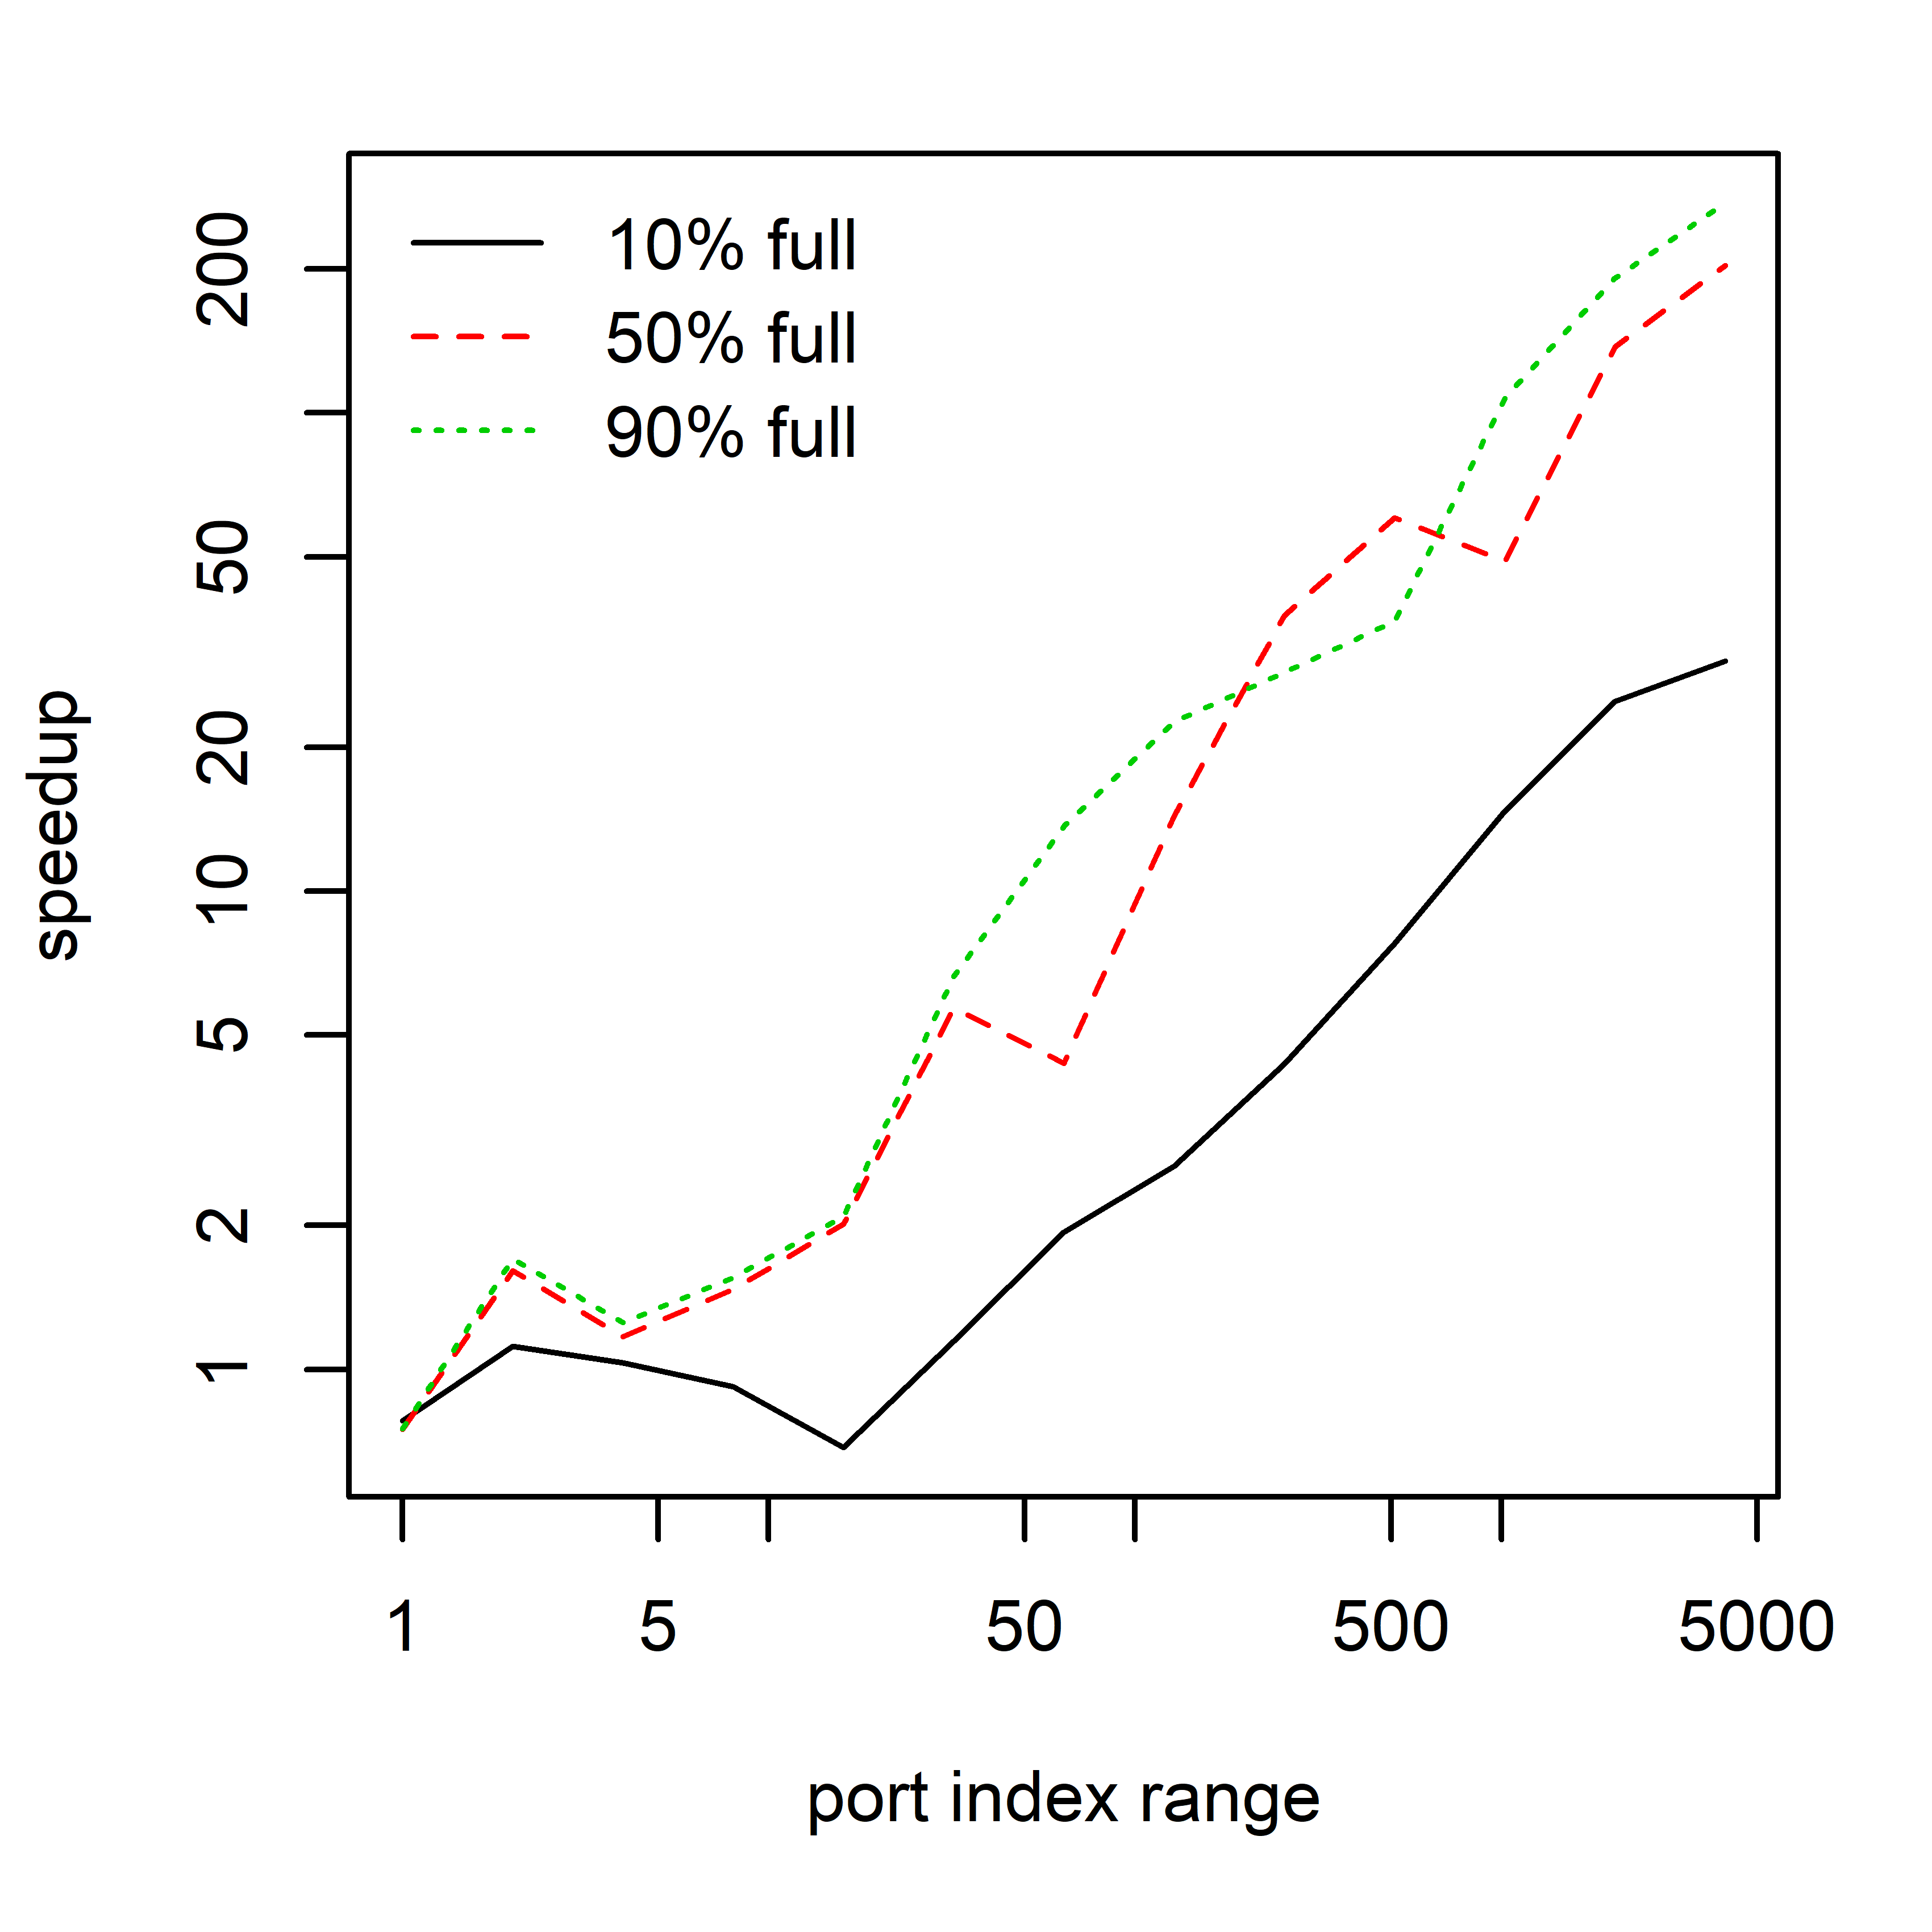
\includegraphics[width=\textwidth]{experiments/bits_1.png}
			\caption{}
			\label{fig:bits_1}
		\end{subfigure}%
	}
	\caption[Bit vector speedup over hashset.]{Run time of the \code{is\_subset} operation for bit vectors and canonical hash sets. This operation is used very frequently by the coordinator to determine whether a rule is satisfied. Figures show (a) run times for the bit vector in response to a changing maximal element, ie.\ number of ports, and (b) the speedup of the bit vector in comparison to the hash set. Note the logarithmic axes.}
	\label{fig:bits}
\end{figure}



The efficiency of the bit vector subset operation is key to the speed of the coordinator. This is the first first three things evaluated for each and every rule, checking whether all involved ports are ready, and if all the relevant memory cells are full or empty. The bit-set capitalizes on how unusually often we need this operation. Figure~\ref{fig:bits} shows how bit vectors are very efficient at checking whether one is a subset of another. Here we see the time taken to evaluate the positive case, representing the best-case scenario for our speedup. It is guaranteed to occur at least three times every time a rule fires. Figure~\ref{fig:bits_0} shows how low the cost of the operation stays, even when there are very many ports involved. Figure~\ref{fig:bits_1} shows how significant the speedup over the subset operation of canonical \code{HashSet} type. Admittedly, the majority of realistic Reo circuits are on the low-end with respect to number of ports; if nothing else, this is a result to encourage the development of more complex connectors. Observe that the cost of the operation is agnostic to the fullness in the case of the bit-vector. This is not so for the hash set, for which a fuller hash set makes for a more expensive operation. 



\subsection{Parallelism Within Interactions}
After data exchanges are initiated by the coordinator, the protocol's lock is released. Time spent exchanging can therefore only impact the threads that play a part directly. Figure~\ref{fig:simo} shows measurements of the $simo$ (`single input, multiple output') protocol, which synchronously distributes a putter's datum to a set of getters. Figure~\ref{fig:simo} shows mean interaction times from the putter's perspective, measured in response to the cost of the data type's \code{clone} operation and the number of recipient getters. For the sake of the experiment, we introduce an artificial \code{clone} operation for our data type, defined such that it spins, performing a predictable amount of bogus value manipulations to simulate some computation of the desired intensity. We use an arbitrary `work unit' as a relative metric of this duration. It's absolute meaning is not necessary; all that matters is that it is defined such that its contribution to runtime is proportionate.

We observe that with fewer than two getters, the runtime does not scale with the work units. Section~\ref{sec:data_exchange} explains that amongst a set of getters, one is elected the \textit{mover}, both responsible for freeing the putter and given permission to move the putter's original if possible. The vast difference made by having any getters at all can be explained by the implementation of the \code{Mutex} type protecting the protocol's critical region. With only one interacting port, the mutex lock is always uncontested, and able to take the `fast path'.\footnote{Our \code{Mutex} comes from the \code{parking\_lot} crate. The relevant documentation is found at~\url{https://amanieu.github.io/parking_lot/parking_lot/struct.Mutex.html}.}

For few work-units, the duration of the interaction was always greater the more getters were involved. Counter to our expectations, this was not a linear relationship. The precise reason for this is uncertain, but owing to its repeatability, we conclude that it's a property of the system used for testing having to share physical cores. Regardless, we observe that for all cases with numerous getters, their durations converge toward more costly clone operations. Figure~\ref{fig:simo_2} confirms that as the parallelizable clone-work increases in significance, getters parallelize their work more effectively.

\begin{figure}
	\centering
	\makebox[\textwidth][c]{
		\begin{subfigure}[b]{0.63\textwidth}
			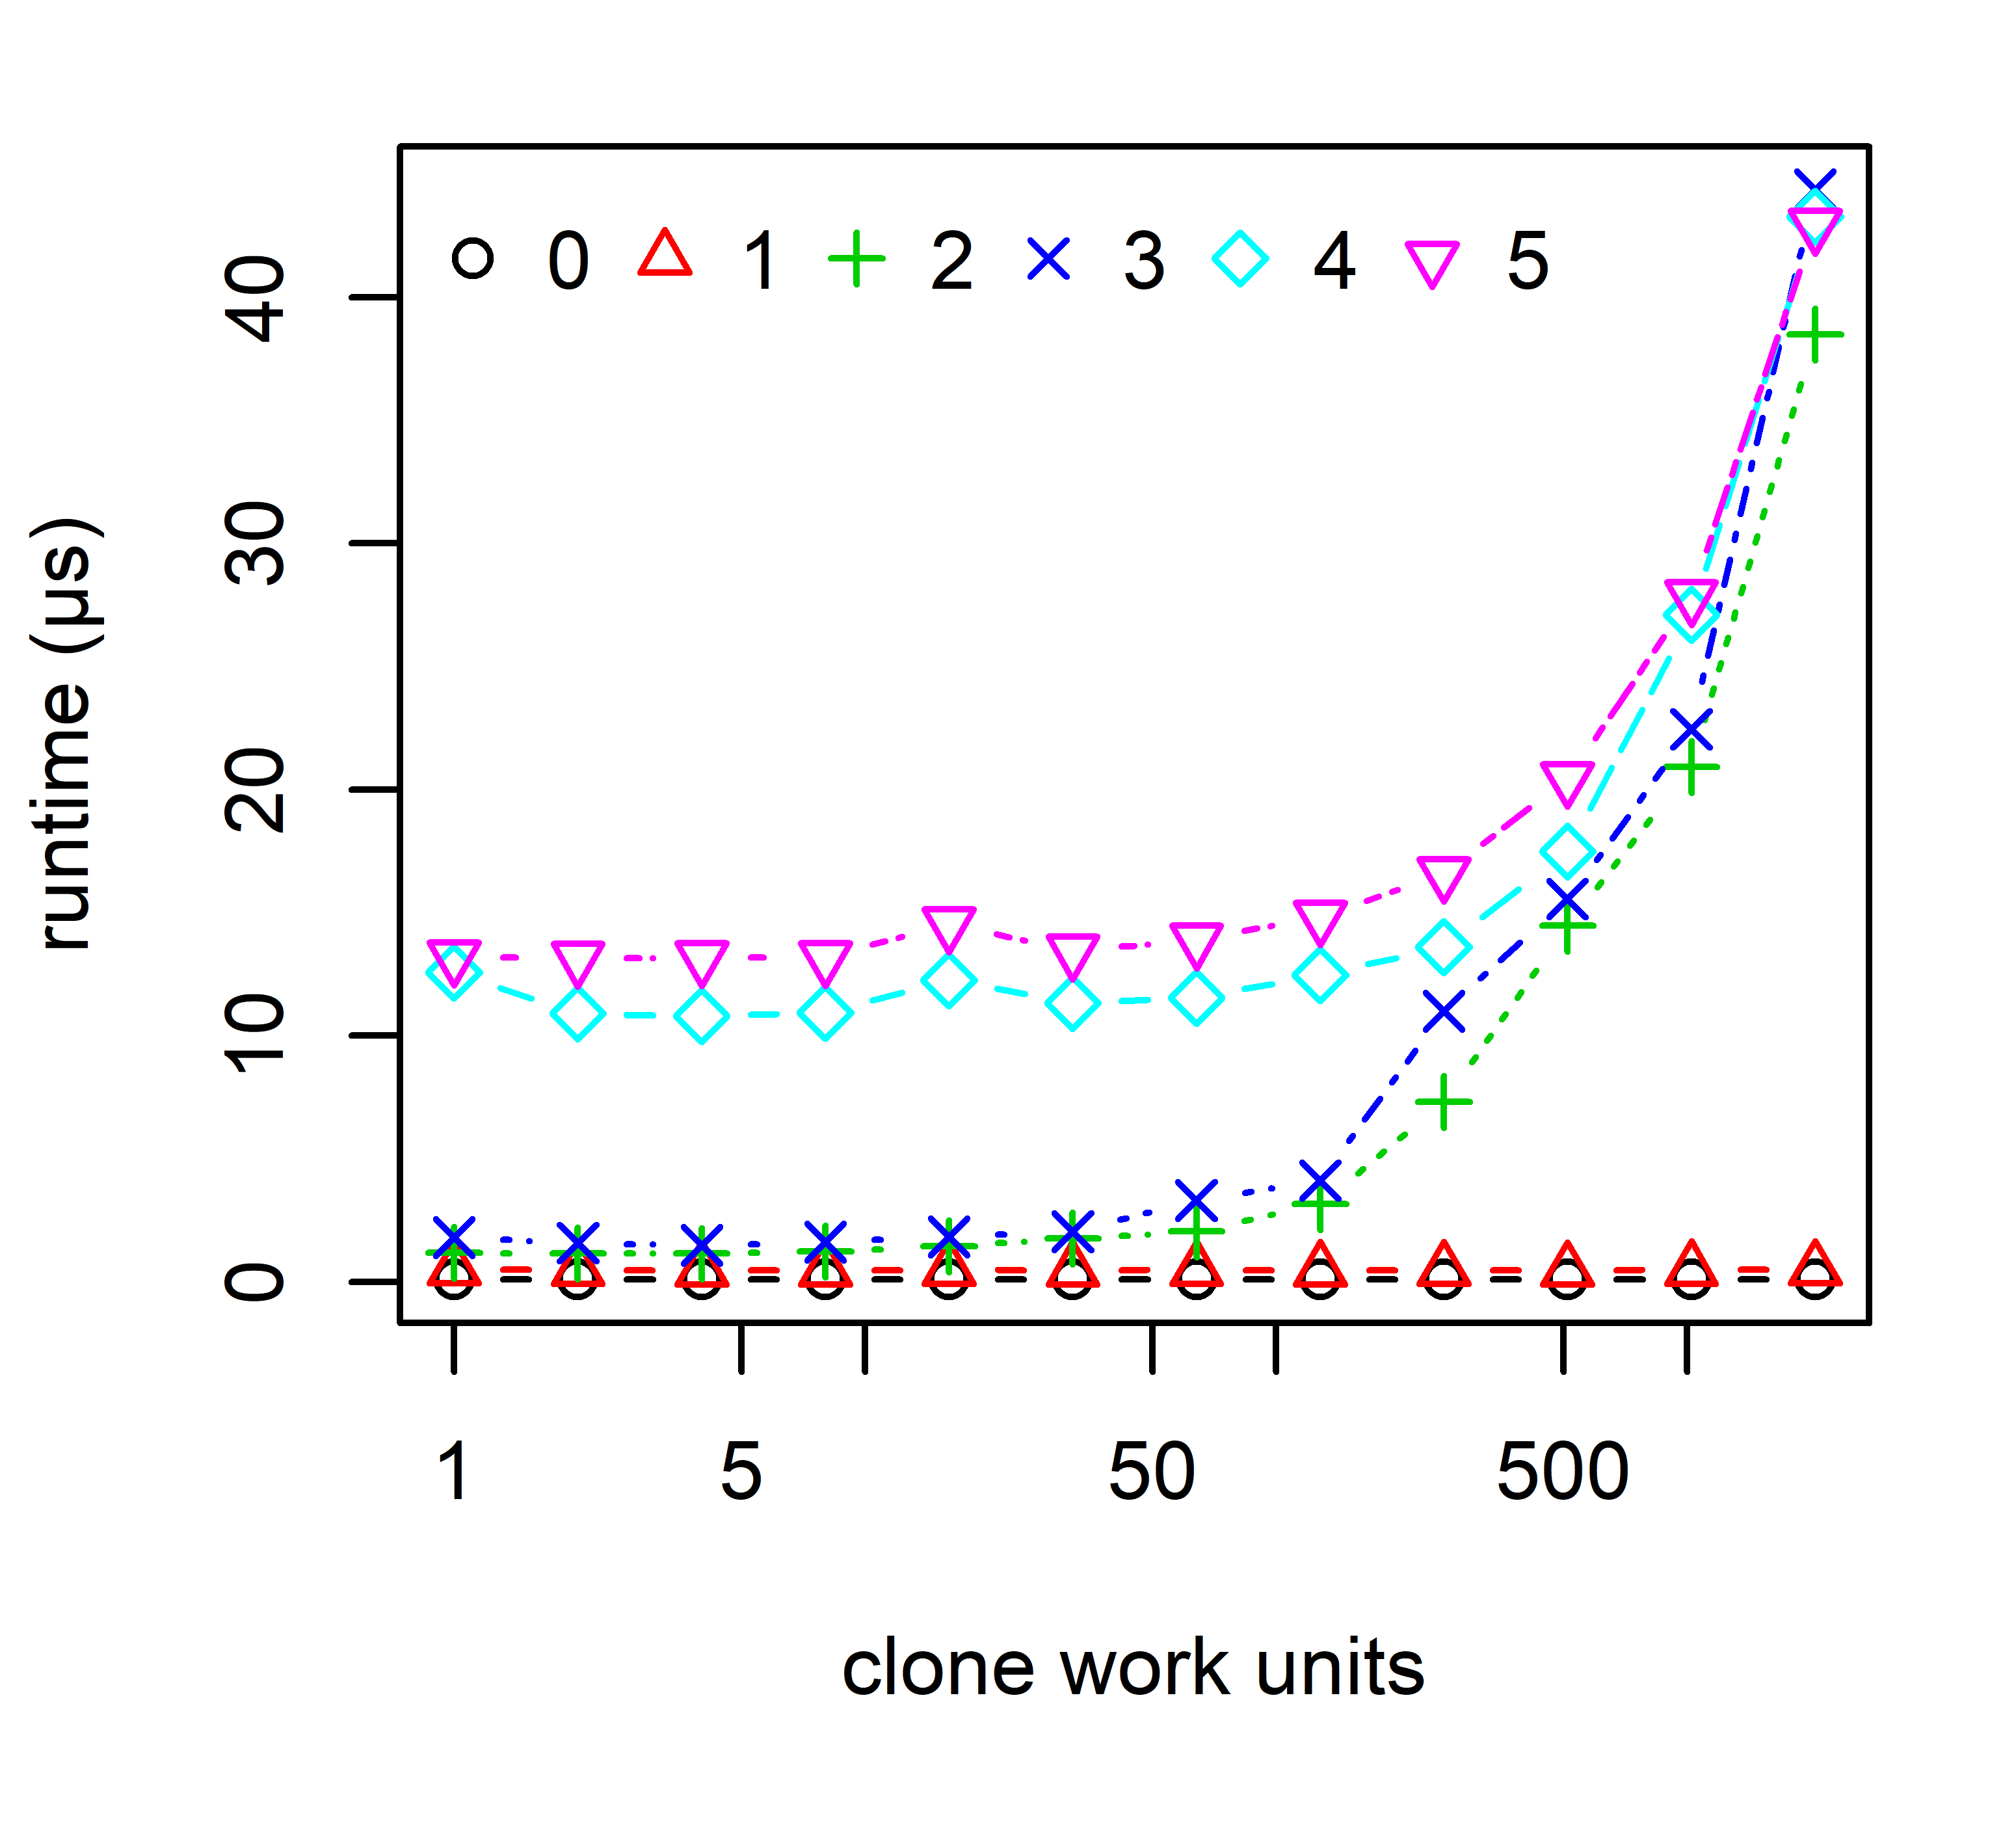
\includegraphics[width=\textwidth]{experiments/simo_0.png}
			\caption{}
			\label{fig:simo_0}
		\end{subfigure}%
		\begin{subfigure}[b]{0.63\textwidth}
			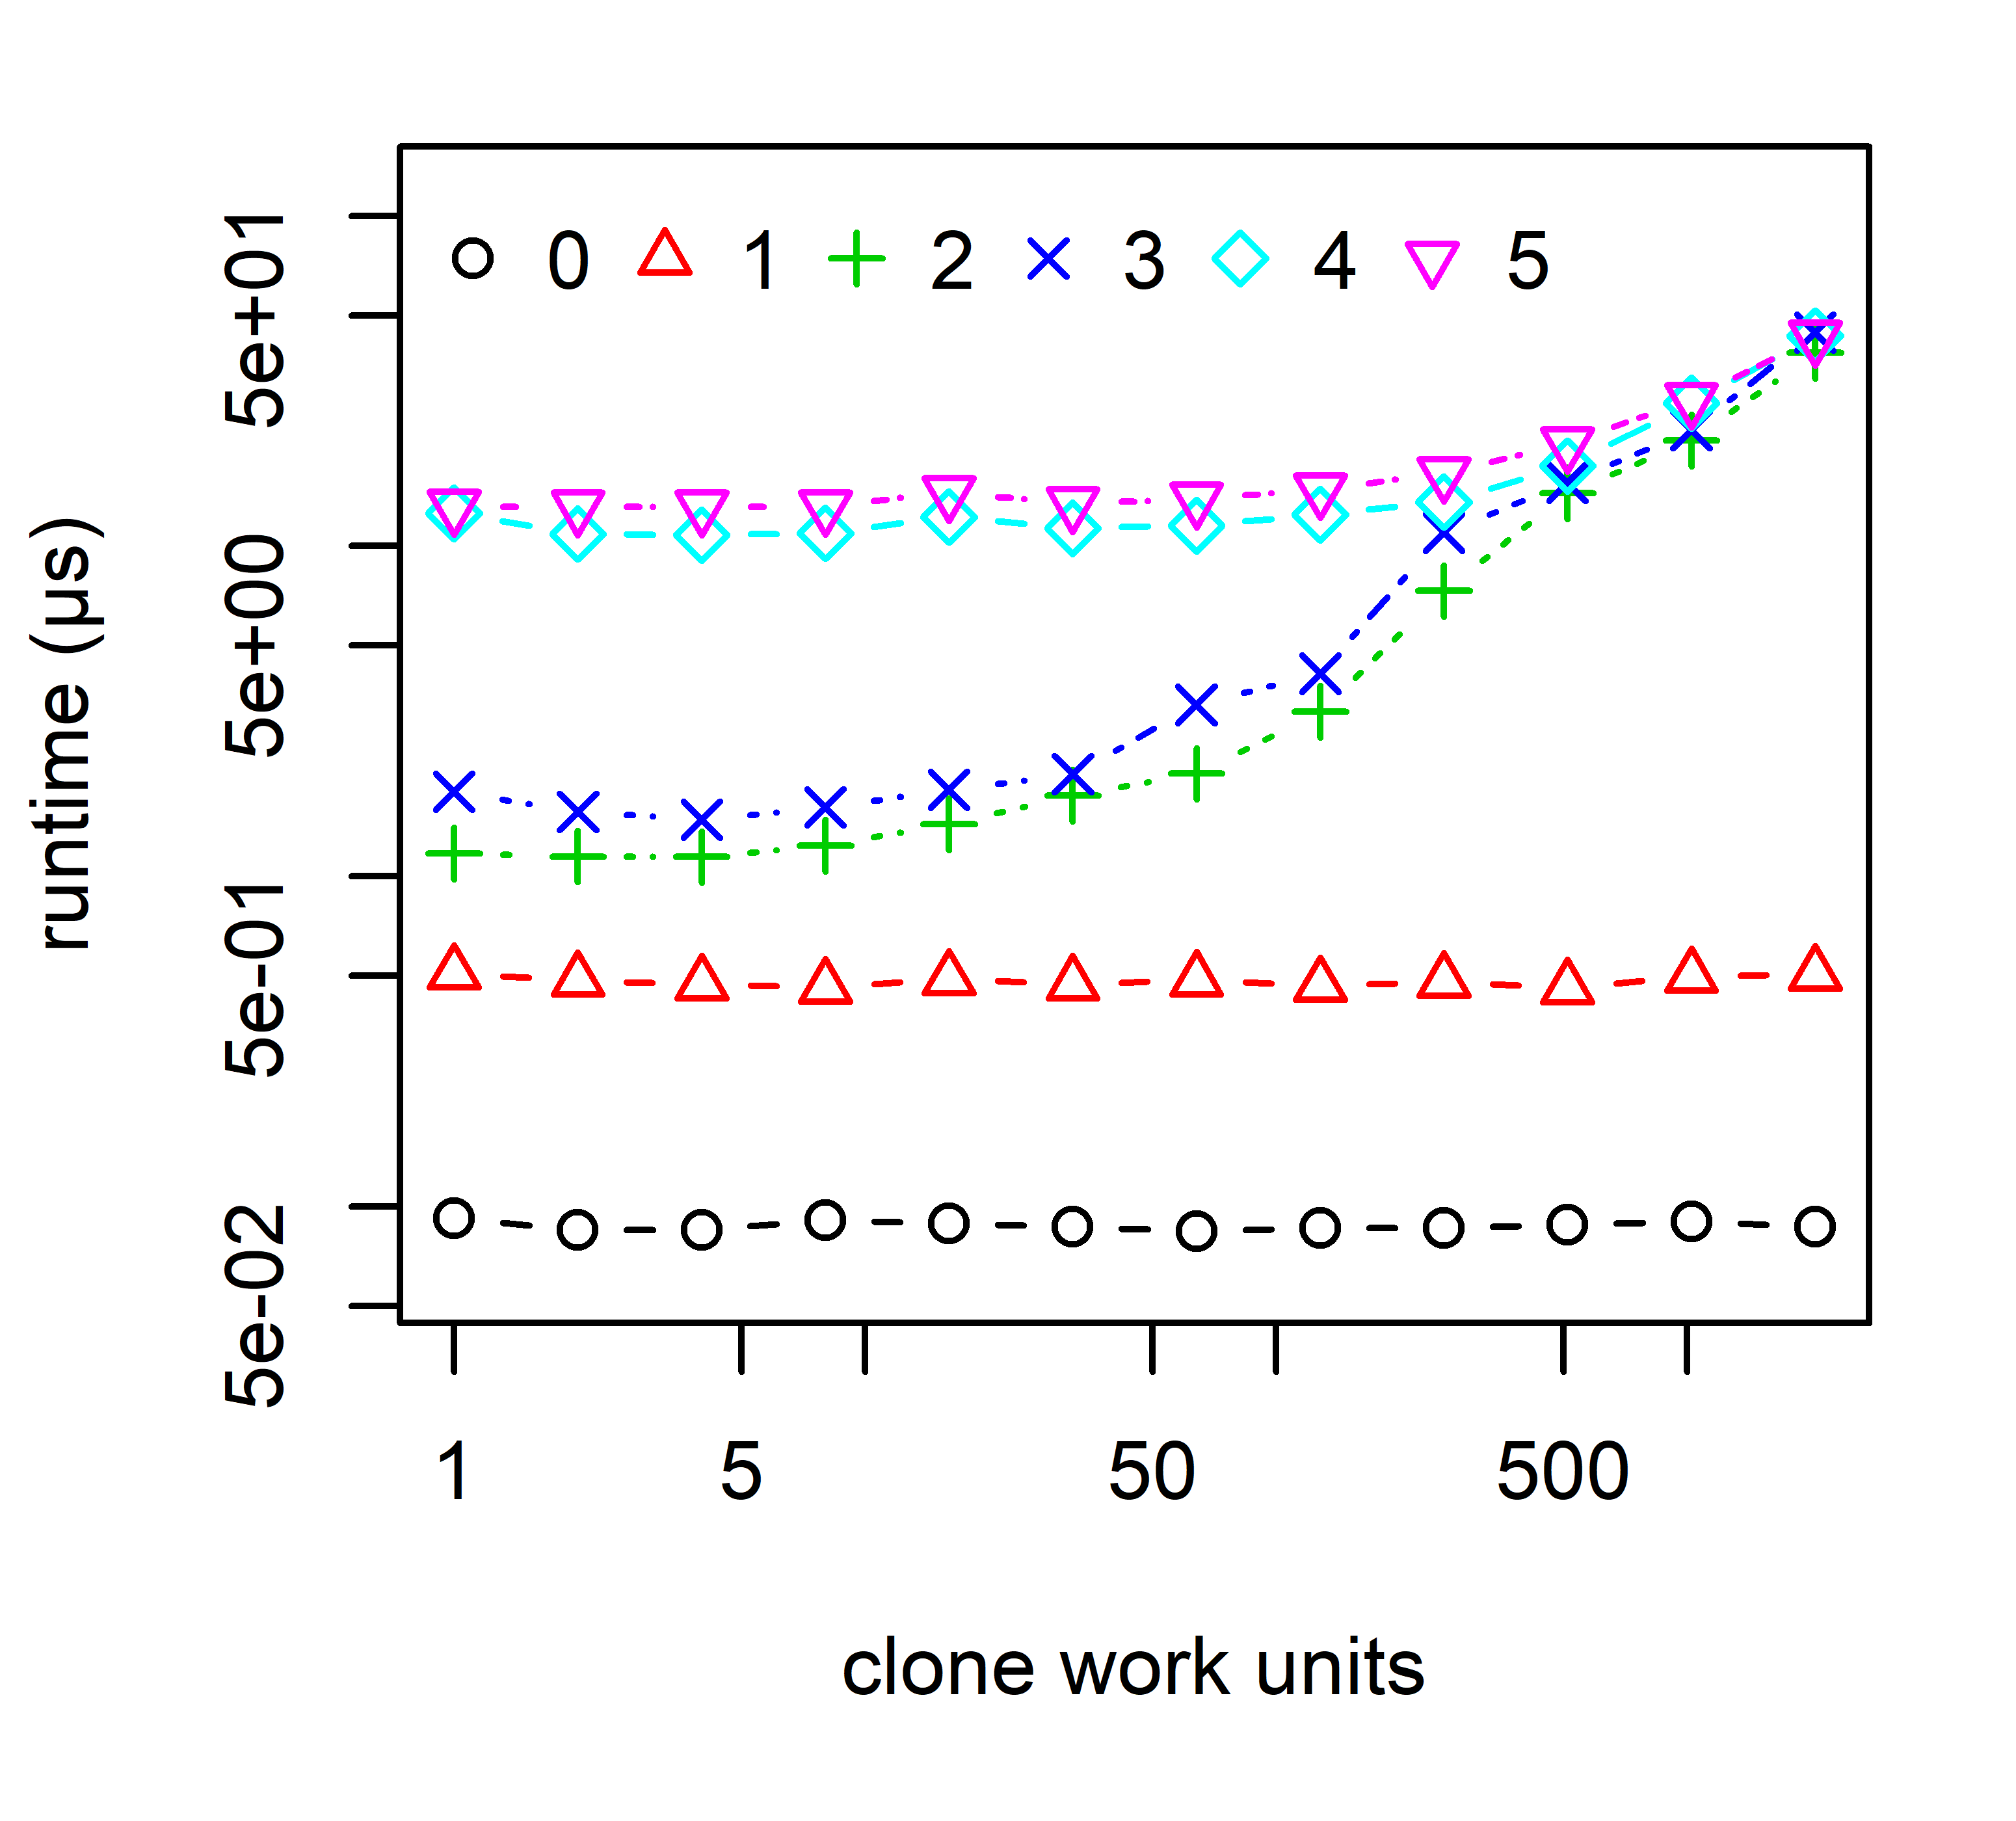
\includegraphics[width=\textwidth]{experiments/simo_1.png}
			\caption{}
			\label{fig:simo_1}
		\end{subfigure}%
	}
	\caption[Interaction duration with parallel getters.]{Mean interaction duration from the perspective of the putter into the $simo$ connector. Results are distinguished by how many getters synchronously acquire the putter's datum in each interaction. Results are shown in response to the cost of the \code{clone} function, in arbitrary \textit{work units}. Note the logarithmic x-axes in both figures, and the logarithmic y-axis in~(b). Measurements are the mean of $100\times{}3000$ repetitions.}
	\label{fig:simo}
\end{figure}


\begin{figure}
	\centering
	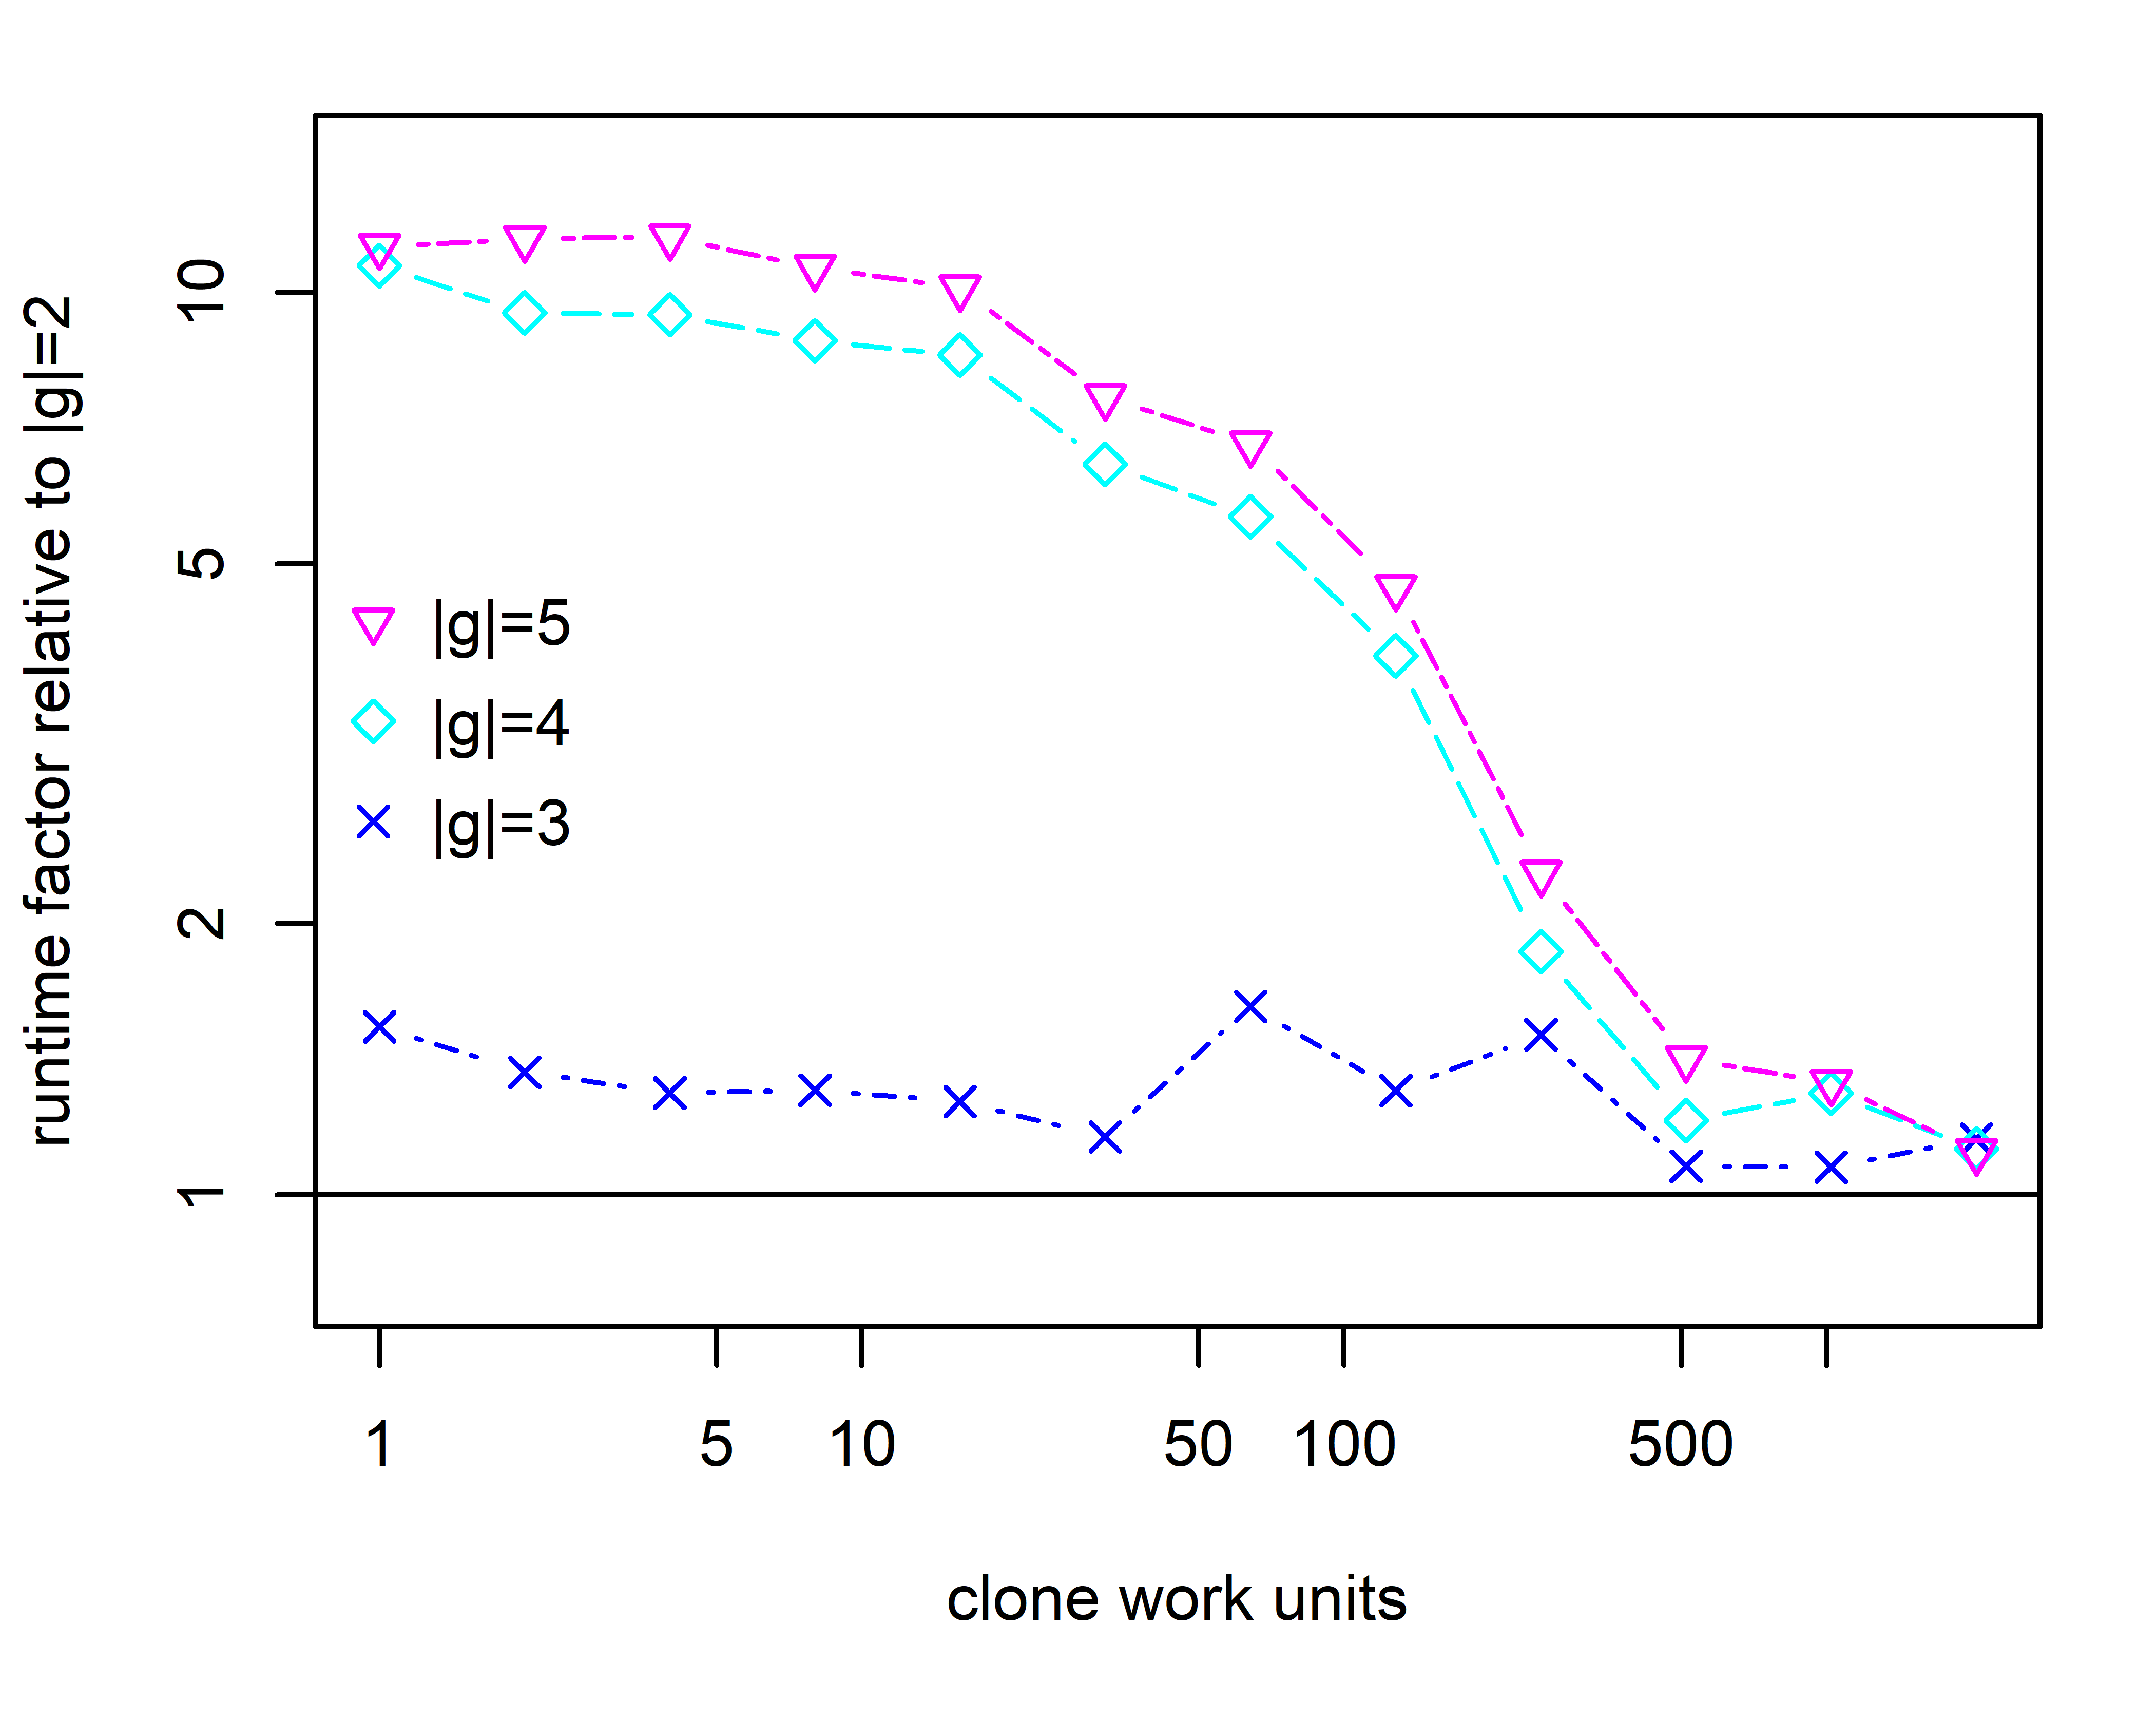
\includegraphics[width=0.80\textwidth]{experiments/simo_2.png}
	\caption[Interaction duration in proportion to the 2-getter case.]{Mean interaction duration in the $simo$ connector, showing slowdown relative to that of runs with two getters. Results are shown in response to the cost of the \code{clone} function, in arbitrary \textit{work units}. Note the logarithmic axes. Measurements are the mean of $100\times{}3000$ repetitions.}
	\label{fig:simo_2}
\end{figure}

\subsection{Reference-Passing Optimization}
Finally, we perform an experiment to verify that the reference-passing optimization described in Section~\ref{sec:memory_cells} is working as intended. Figure~\ref{fig:fifo_m} shows the results of the mean time taken for a datum to pass through a $fifoN$ connector. This protocol makes trivial use of an $m$-long chain of memory cells. Values originate as input on one end, shifting between cells from head to tail, and finally being output at the tail. All measurements are dominated by the work of moving the $2^{13}$-byte values in memory from one place to another. \texttt{shift\_get} represents the most intuitive run, where values are moved twice: once \textit{into} the protocol's storage, and once \textit{out} to the getter. For this protocol, the Rust compiler failed to optimize the logical data-movement of the safe API's \code{put} operation. Runs using this safe variant are prefixed with~\texttt{put\_}, and include an additional value-movement.

As expected, runtimes in Figure~\ref{fig:fifo_m_0} are seen stratified according to the number of movements they perform. In all cases, longer chains of memory cells indeed require more time (preventing the runtime to be constant with respect to~$m$), but the overhead is relatively small, and does not appear to be affected by the baseline cost of movement; this is expected, as the cost of reference-passing is unrelated to the value's size, or data type in any way.

Figure~\ref{fig:fifo_m_1} shows how the cost of reference-passing compares to the best- and worst-case scenarios for the response of interaction time to the length of the chain. Previously we have observed that Reo-rs experiences some constant overhead per port interaction (eg.\ in Figure~\ref{fig:exper_rtt_1}), so interaction time would likely remain sublinear even if it performed value-passing between memory cells na\"ively. However, in most examples (including this one) we can safely presume it's slope would be far steeper than it is now.

\begin{figure}
	\centering
	\makebox[\textwidth][c]{
		\begin{subfigure}[b]{0.63\textwidth}
			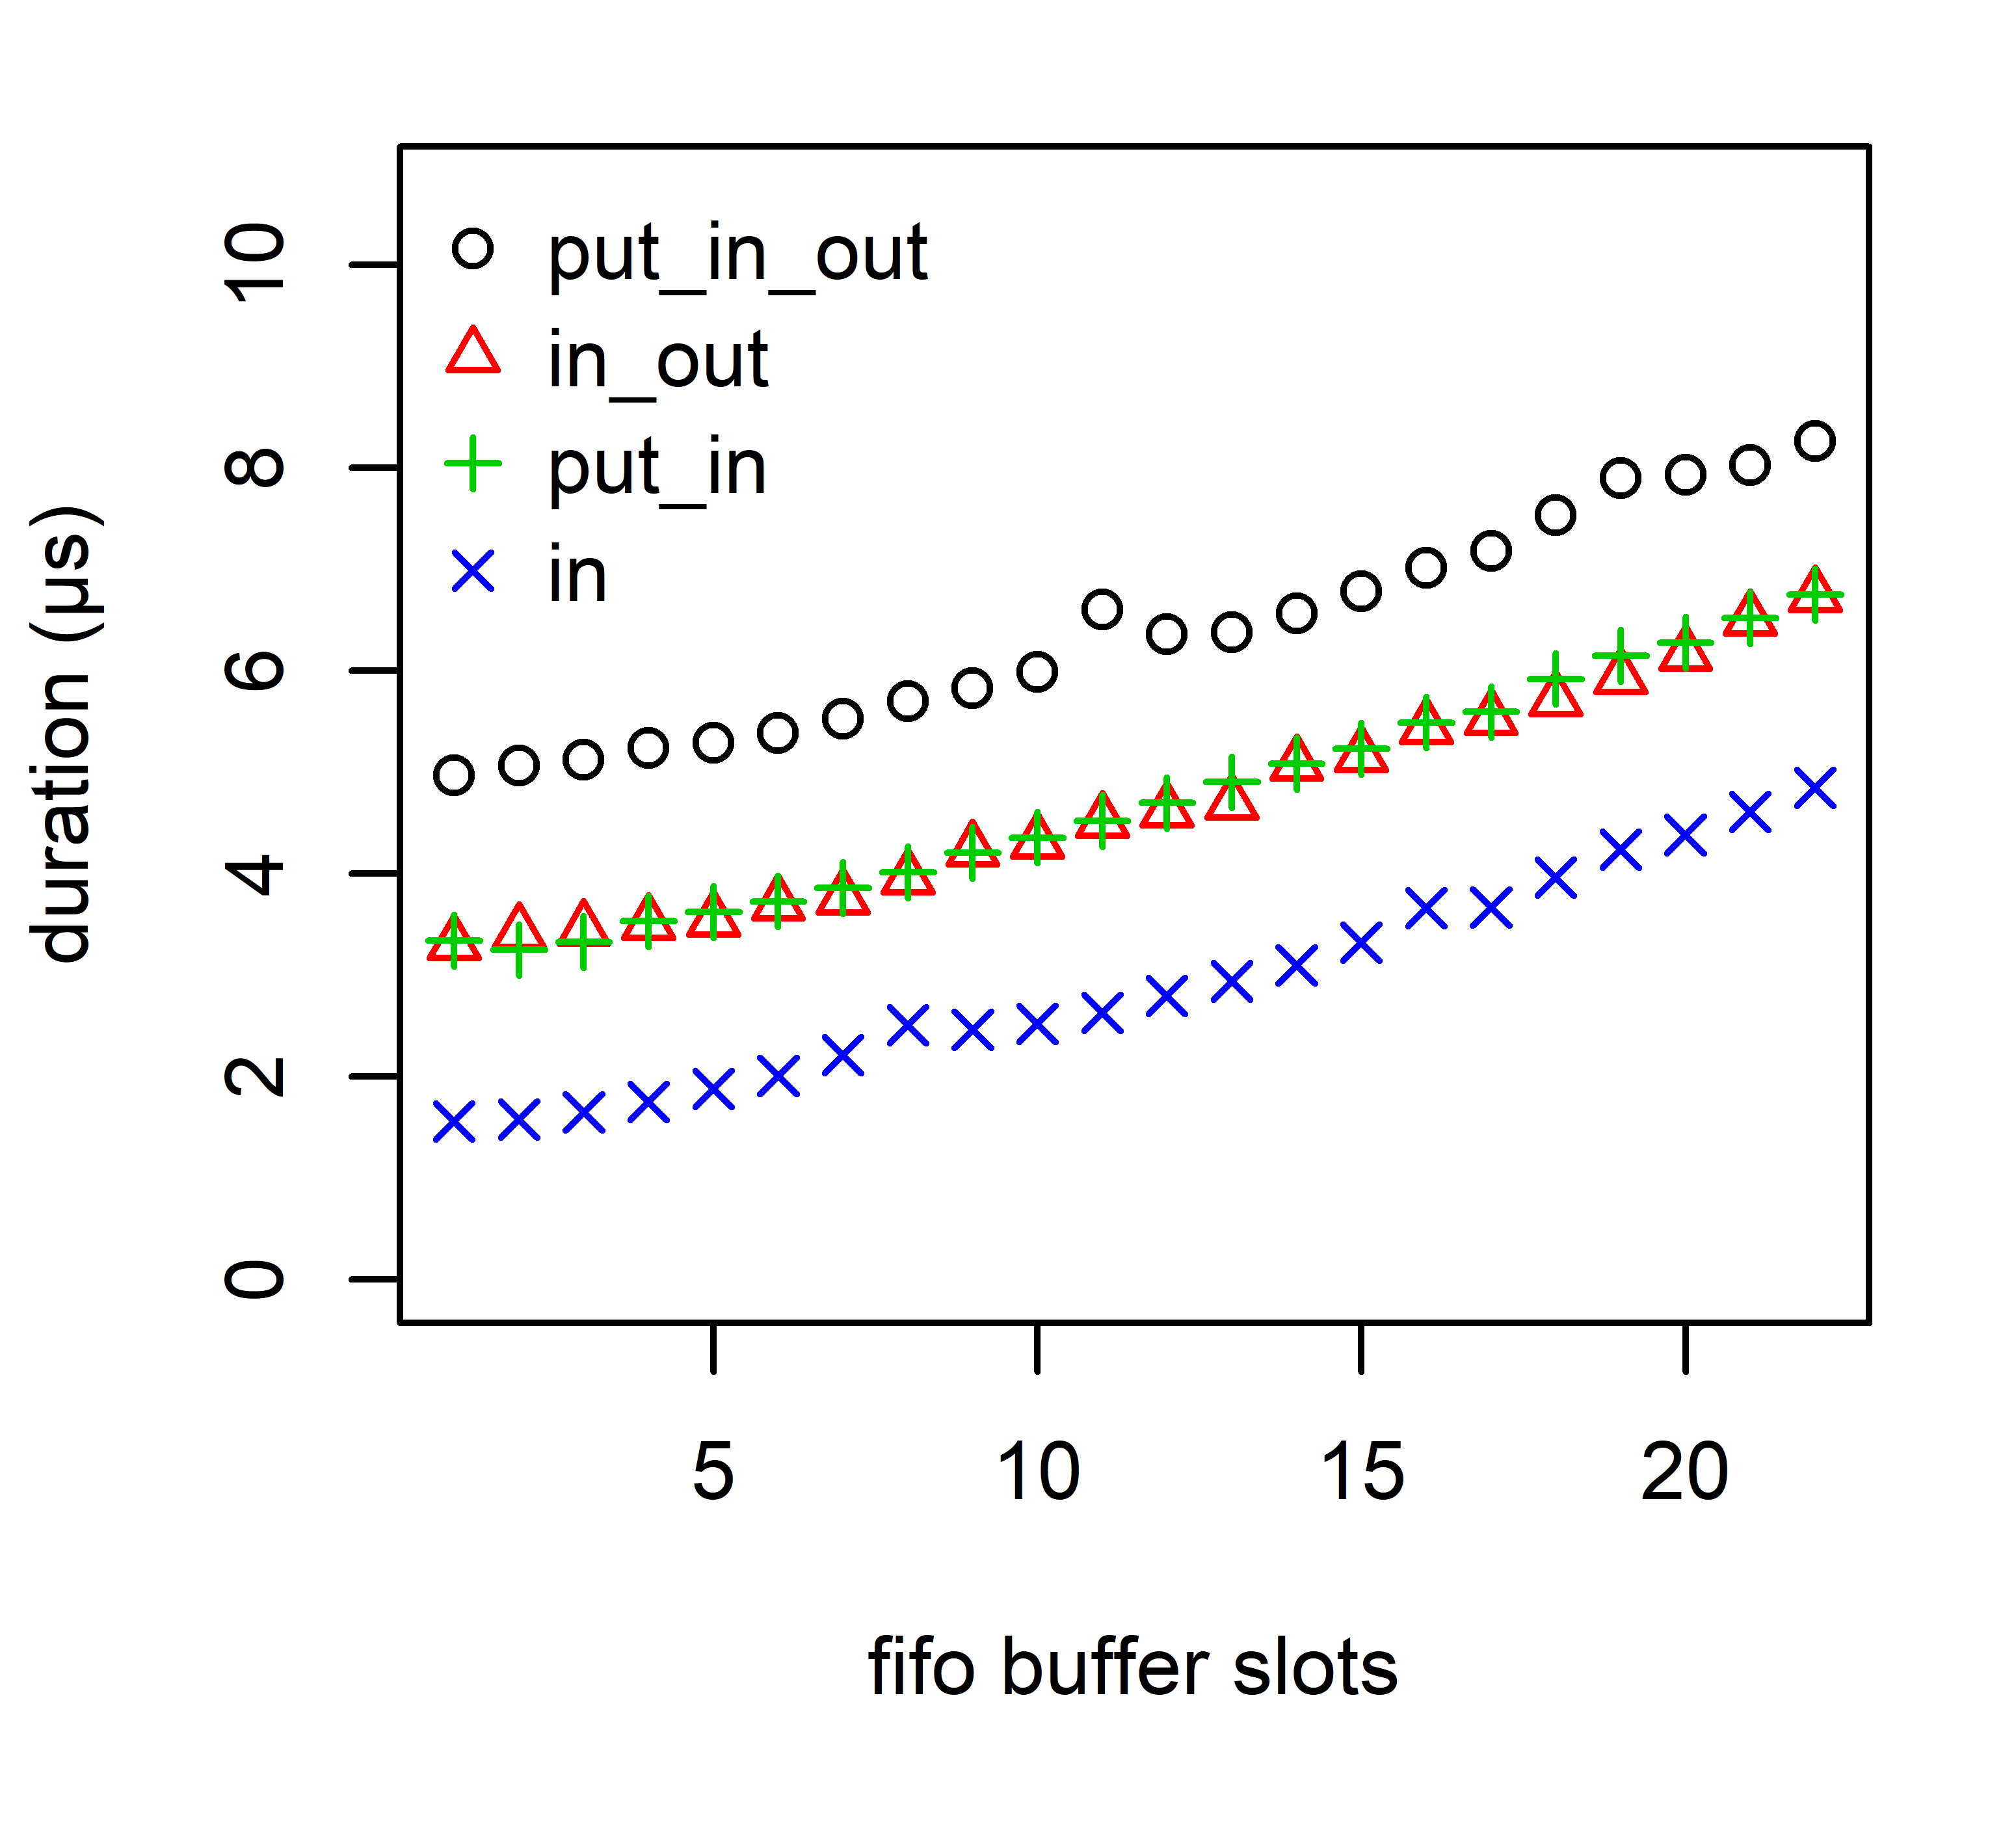
\includegraphics[width=\textwidth]{experiments/fifo_m_0.png}
			\caption{}
			\label{fig:fifo_m_0}
		\end{subfigure}%
		\begin{subfigure}[b]{0.63\textwidth}
			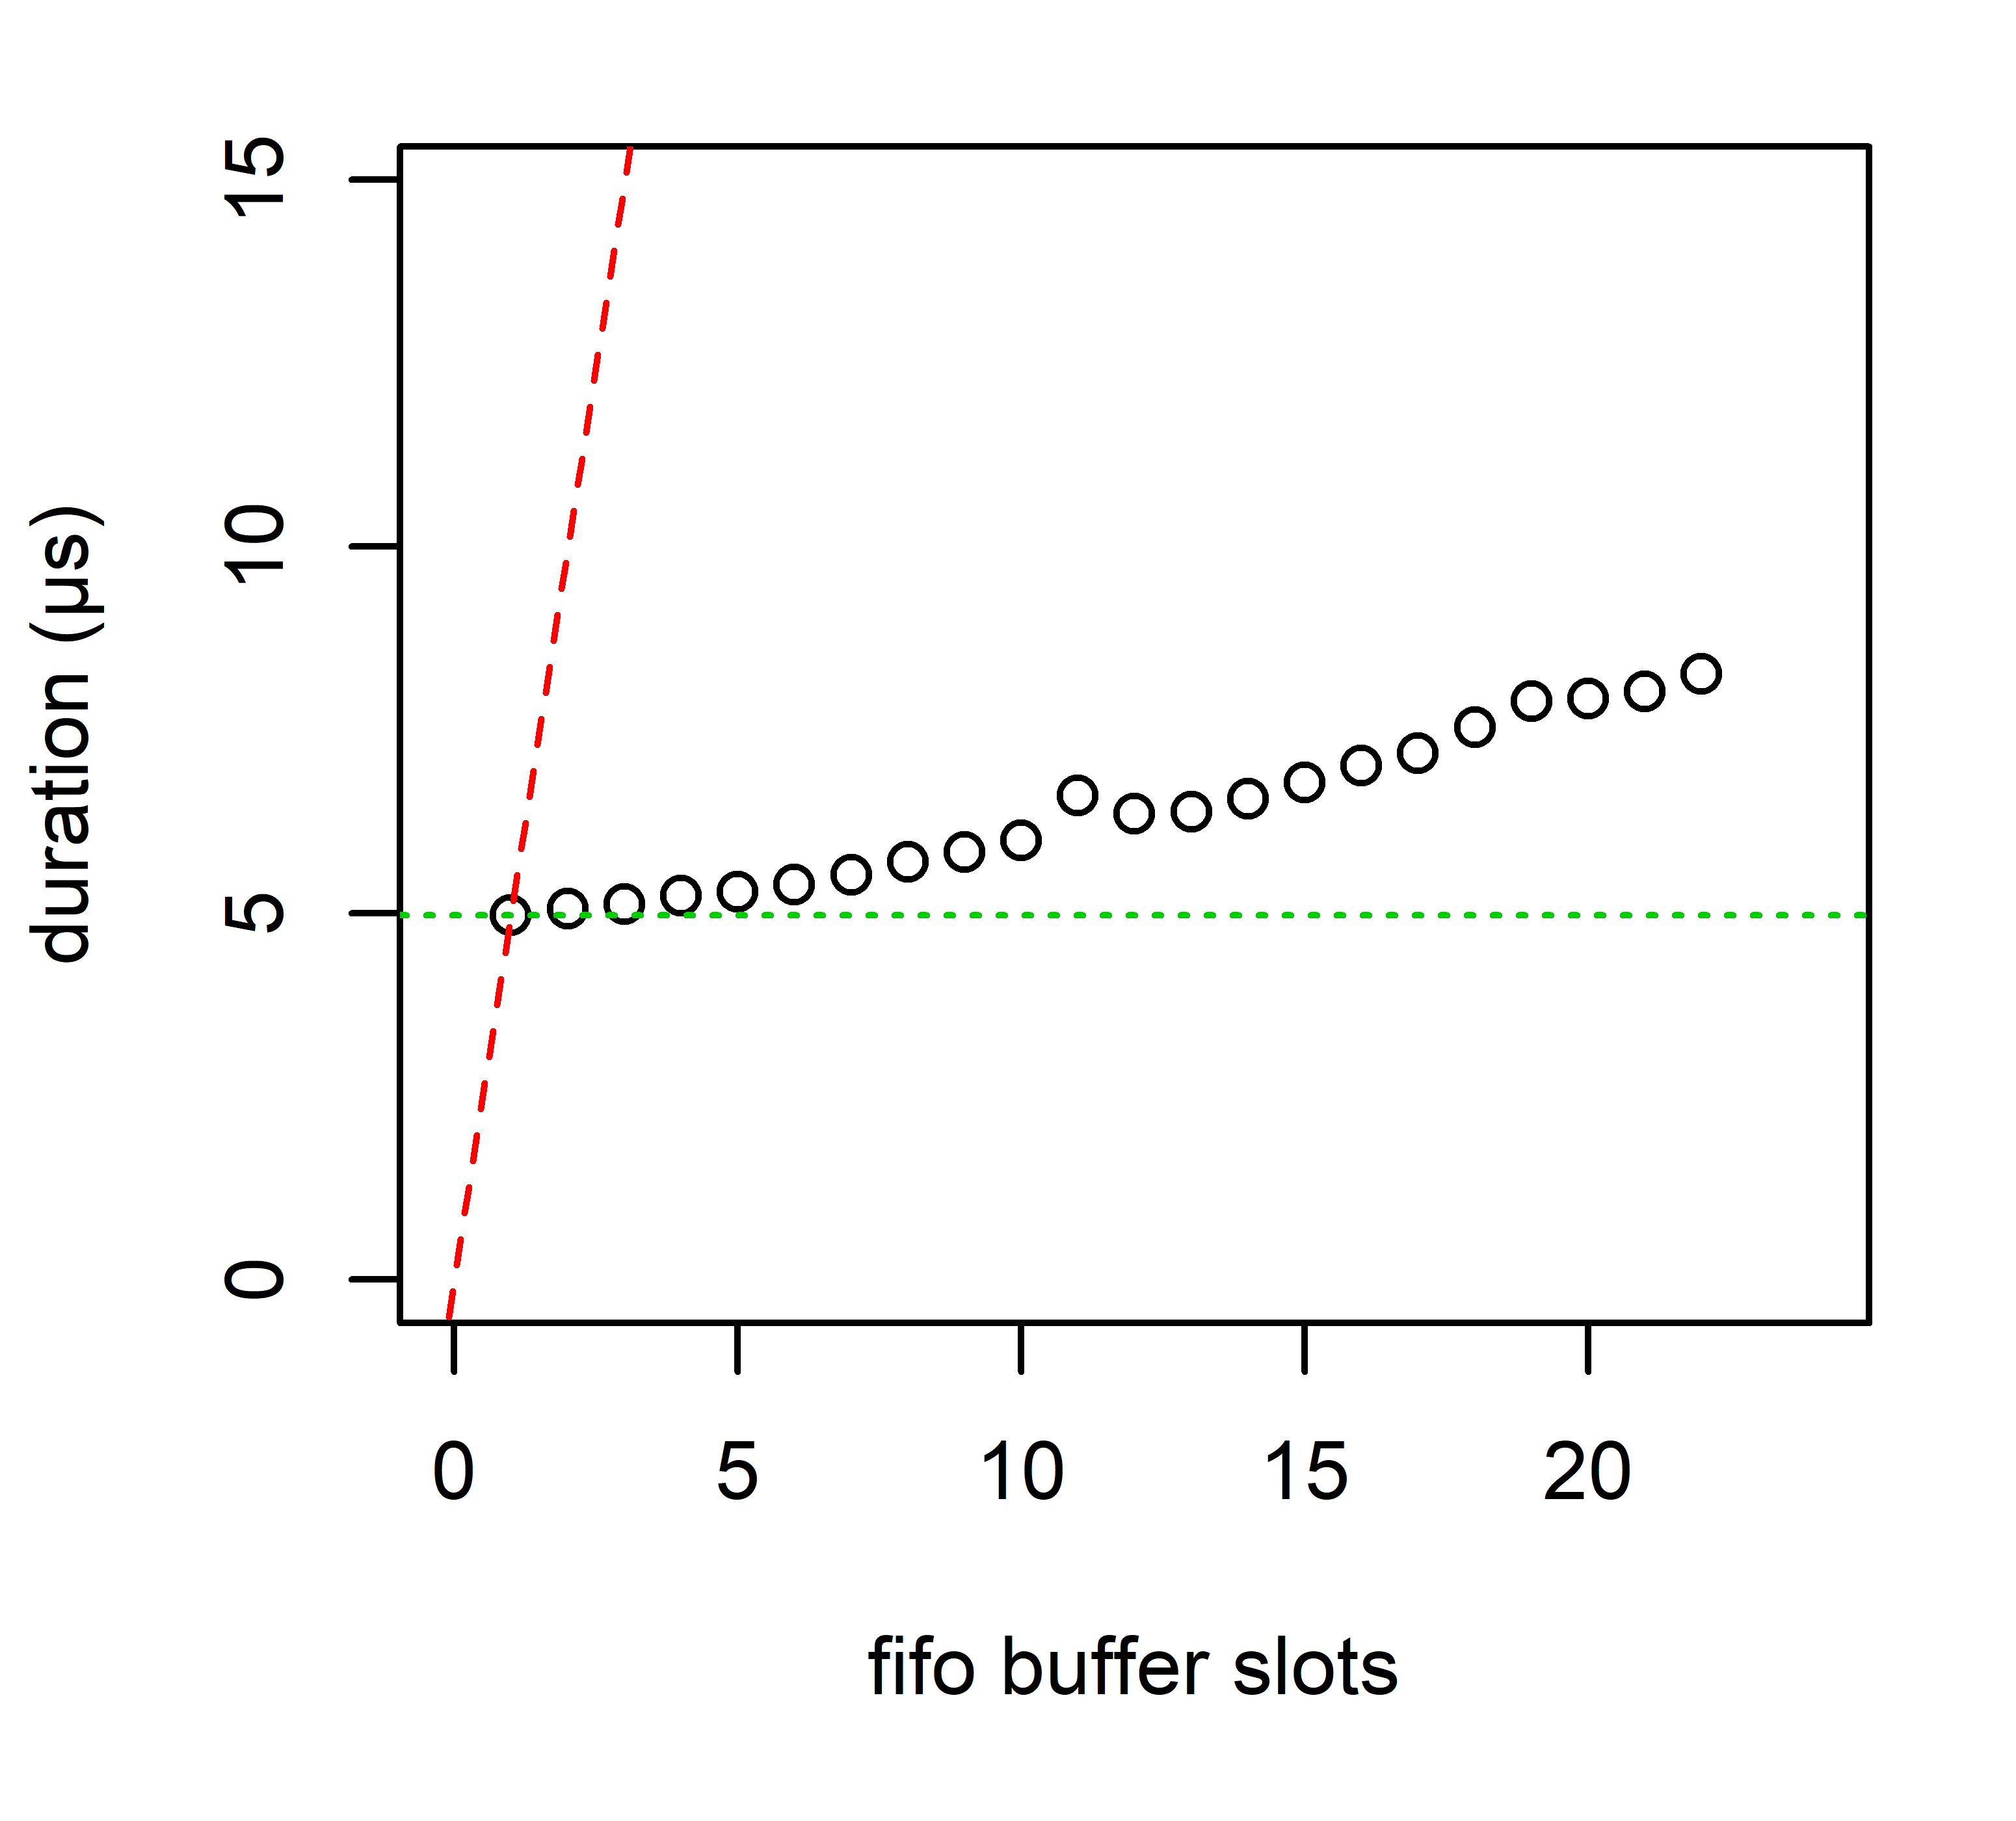
\includegraphics[width=\textwidth]{experiments/fifo_m_1.png}
			\caption{}
			\label{fig:fifo_m_1}
		\end{subfigure}%
	}
	\caption[RTT for fifoN connector with $2^{13}$ byte values.]{Round trip time (RTT) of a $2^{13}$ byte value through a $fifoN$ connector with~$m$ ranging from 1 to 20, measuring the time taken from the start of the~\code{put} into the head of the chain, to the end of the \code{get} out of the tail. (a)~The experiment was repeated using variations of port operations to control the number of memory copies. \texttt{put\_*} runs move the datum using the safe value-passing API, and others use the unsafe C-like reference-passing API. \texttt{*\_get} runs acquire the output by value, while others participate in synchrony by acquiring a signal. (b)~\texttt{put\_in\_out} is compared to the best- and worst-case scenarios for interaction times in response to~$m$. Measurements are the mean of $100\times{}10~000$ repetitions.}
	\label{fig:fifo_m}
\end{figure}
